% !TeX root = ../libro.tex
% !TeX encoding = utf8


\chapter{Resultados de frenado magnético de intensidad variable}\label{ch:septimo-capitulo}
\section{Configuración de los modelos} \label{marco_teorico_ii}

A COMENTAR
Parametrización de los modelos
Rango de valores a asignar a los parámetros libres
Ciclo de control
Para cada paso de simulación
- Obtenemos o calculamos la intensidad del campo magnético
- Calculamos la pérdida de momento angular inducida por el campo magnético
- Distribuimos la pérdida de momento angular entre las capas de la estrella
- Obtenemos o calculamos el valor de $\amlt$


\section{Modelos de evolución estelar}
Como venimos exponiendo en el capítulo anterior, con la consideración de campos magnéticos de intensidad variable ($B$) dependientes de los parámetros estelares $\Omega$ y $\teff$ llevamos nuestra línea de trabajo un paso más allá. La parametrización base utilizada es básicamente la misma que hemos utilizado al abordar los campos magnéticos de intensidad fija. La innovación fundamental radica en la introducción de una intensidad de campo magnético variable ($B$) y un parámetro $\amlt$ variable. En cuanto al tratamiento de la mezcla convectiva con sobreimpulso (overshooting), es evidente una desviación del modelo anterior; desactivamos deliberadamente esta característica en nuestro modelo actual. Esto aísla el impacto de una variable $\amlt$ en A(Li) de los efectos asociados con el sobreimpulso convectivo. En particular, la mezcla convectiva con sobreimpulso se aborda habitualmente mediante extensiones ad hoc de la Teoría de la Longitud de Mezcla (MLT), introduciendo así un parámetro libre adicional. La Tabla \ref{tab:phy_mesa_ii} enumera las similitudes y diferencias en la configuración de los modelos utilizados en \cite{Caballero2020} y en este trabajo.\par

\begin{table}
	\begin{threeparttable}
		\centering
		\begin{tabular}{ll} 
			\hline
			Parámetro & Prescripciones y valores adoptados\\
			\hline
			Abundancia Solar & $X_{\odot}=0.7154, Y_{\odot}=0.2703, Z_{\odot}=0.0142$\\
			Ecuación de estado & OPAL+SCVH+MacDonald+HELM+PC\\
			Opacidad & OPAL Tipo I para log T $\geq$ 4 \\ & Ferguson para logT $<$ 4\\
			Tasas de Reacción & JINA REACLIB\\
			Condiciones de Contorno & ATLAS12; $\tau$=100 tablas + fotoesfera\\
			Difusión & Rastreo de \isotope[1]{H}, \isotope[2]{He}, \isotope[7]{Li}, \isotope[7]{Be}\\
			Esquema de Rotación & Rotación diferencial en PMS \& MS\\ & Incluye SH\tnote{1}  , ES\tnote{2}  , GSF\tnote{3}  , SSI\tnote{4}  , DSI\tnote{5}\\
			Termohalina & $\alpha_{\textrm{th}}=666$\\
			\textbf{Convección} & $\alpha_{\textrm{MLT}}$ variable dependiente de $\teff$\\ & \& $\gsurf$ + Ledoux\\
			Semiconvección & $\alpha_{\textrm{sc}}=0.1$\\
			\textbf{Sobreimpulso} & $f_{\textrm{ov,core}}=0.0$, \& $f_{\textrm{ov,sh}}=0.0$\\
			\textbf{Campo Magnético} & B(G) variable, dependiente de $\rho$, $\teff$ \&  $\Omega$\\
			Pérdida de Masa & $\Dot{M}_{\textrm{max}} = 10^{-3} \: \msun \: yr^{-1}$\\
			Périda de Momento Angular & $\Dot{J} = \Omega_* \; \mwind \; \ralfven^2$\\
			\hline
		\end{tabular}
		\begin{tablenotes}\footnotesize
			\item (1) Solberg-Hoiland, (2) Eddington–Sweet
			\item (3) Goldreich–Schubert–Fricke, (4) Secular Shear Instability
			\item (5) Dynamical Shear Instability
		\end{tablenotes}
	\end{threeparttable}
	\caption{Resumen de la física adoptada en MESA \cite{Choi2016,Caballero2020}[basado en][]. Resaltados en negrita los parámetros con diferente configuración de los trabajos referenciados.}
	\label{tab:phy_mesa_ii}
	
\end{table}


Los modelos incluyen rotación desde el PMS. Hemos calculado la evolución de modelos estelares de $1\,\msun$ en metalicidad inicial solar con $\omegaini = \oomegac$ que varía entre $0.12$ y $0.1425$. A continuación, los resultados se comparan con las edades estelares de estrellas en OC recogidas por la misión Gaia y GES y referenciadas en la Tabla \ref{tab:oc_reduced_list}.\par

\subsection{Evolución del Li con MB de intensidad variable}
Existen evidencias que abogan por una fuerte relación establecida entre la destrucción de Li y la rotación estelar, de forma que cuanto mayor es la velocidad angular, mayor es la destrucción de Li (ver \cite{Bouvier2018, Caballero2020}). El efecto del MB en la evolución temporal de A(Li) viene dado por su capacidad para eliminar AM de la estrella, y por tanto influir en su velocidad de rotación, haciendo que la estrella rote más lentamente y destruya menos Li.\par

En la figura \ref{fig:li_var_vel_var_g_3} se muestra la evolución temporal de la abundancia superficial de Li para varios modelos de 1 $\msun$. Estos modelos se inicializaron con diferentes velocidades de rotación y tuvieron en cuenta los efectos del MB causado por un campo magnético variable. Si lo comparamos con la Figura \ref{fig:li_var_vel_0g} en la que se despreciaron los efectos del MB, observamos cómo se alteraron los perfiles de abundancia de Li a lo largo del PMS y el MS. Durante el PMS podemos describir el efecto como modesto, algo esperado y en línea con el hecho de que el AML causado por MB (ver Ec.~\ref{eq:j_dot}) depende directamente de la evolución de $\Omega$ y de la tasa de pérdida de masa. Si tenemos en cuenta que para las estrellas de tipo solar los modelos predicen una tasa de pérdida de masa total modesta, ese valor es incluso mucho menor en esta fase. Es en la fase de aproximación a la ZAMS cuando la velocidad angular alcanza su máximo. Esto, según nuestro modelo, desempeña un papel crucial tanto en la pérdida de masa como en la intensidad del campo magnético. Cuanto mayor sea $\Omega$, mayor será $\Dot{M}$ (véase la Figura \ref{fig:mdot_var_vel_g3}), y mayor será la intensidad del campo magnético (véase la Figura \ref{fig:mag_field_var_vel_g3}). Estos efectos se combinan y conducen a una acentuación del efecto de frenado magnético. Como consecuencia, se produce una ralentización de la destrucción del Li una vez que los modelos entran en el EM. Los resultados de nuestras simulaciones para esos modelos inicializados respectivamente a $\omegaini$ = 0.14 y 0.1425 reproducen A(Li) en línea con la de la abundancia del \isotope[7]{Li} de la superficie del Sol (1,1 $\pm$ 0,1 dex). Este último da un valor de 1,133 dex, lo que representaría una desviación de aproximadamente el 3\% del valor nominal (véase la Figura \ref{fig:li_var_vel_var_g_3}).\par

\begin{figure}
	\centering
	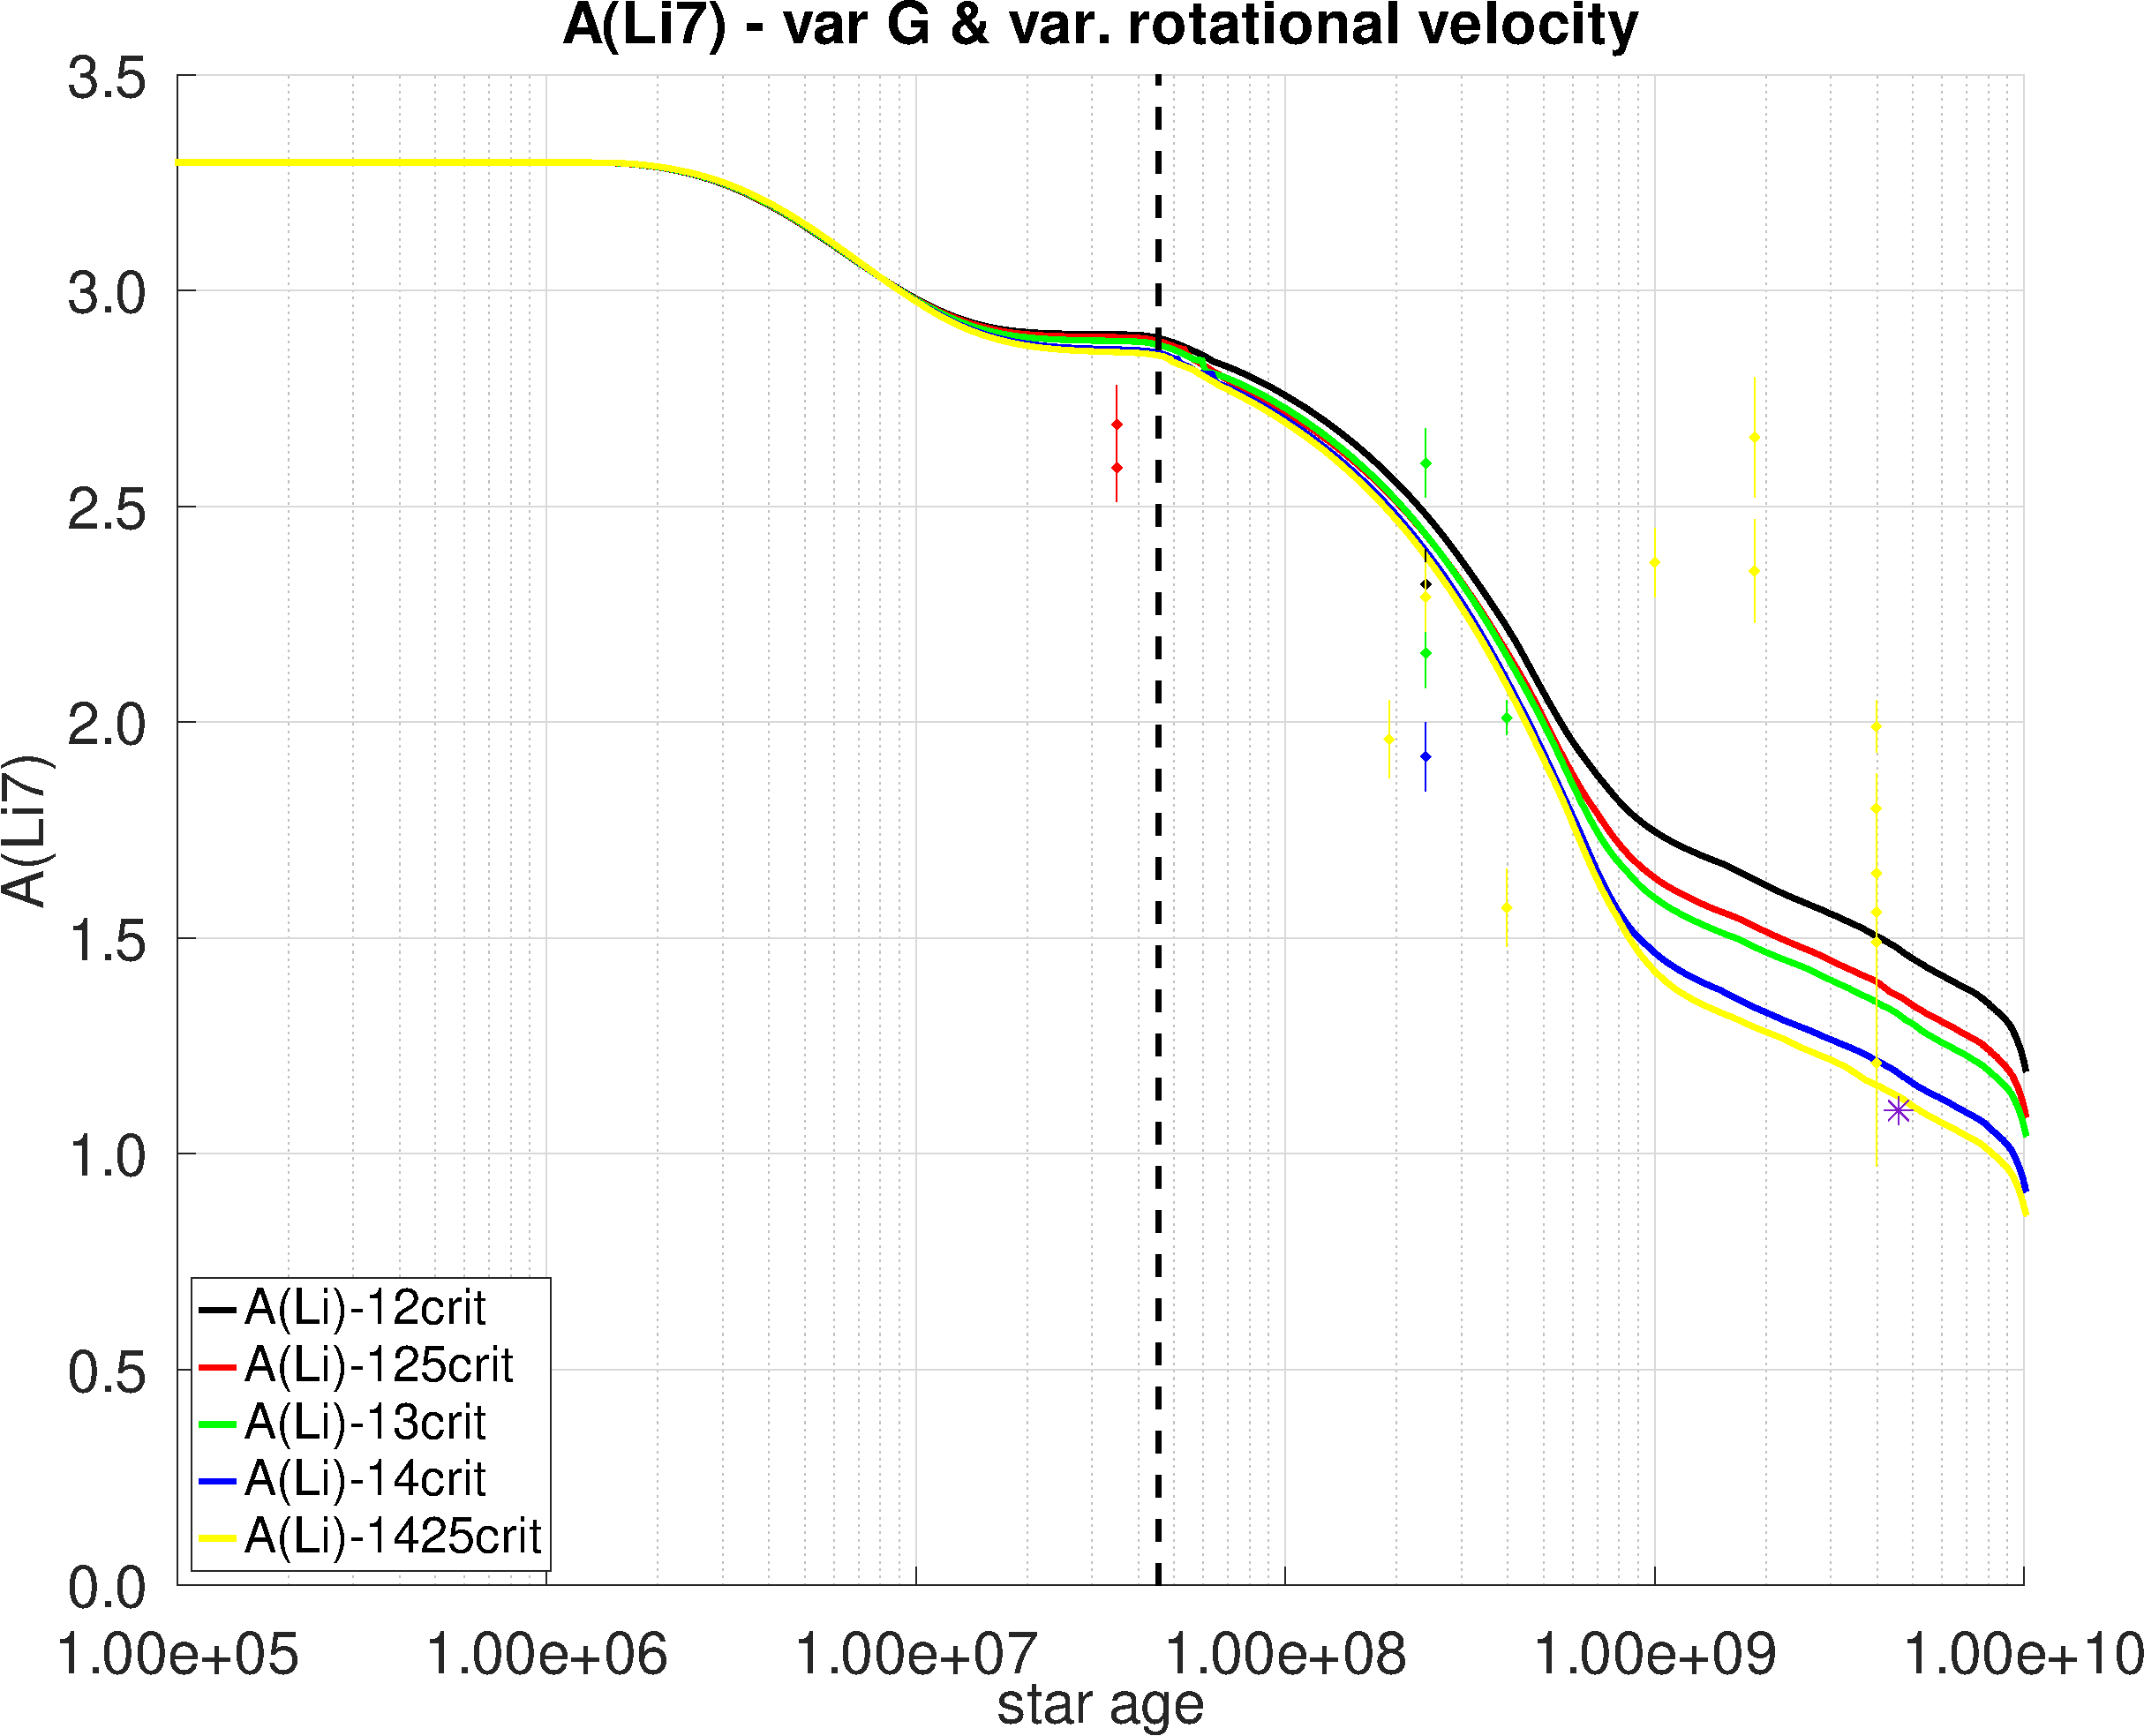
\includegraphics[width=0.7\textwidth]{img/paper2/li_var_vel_var_g_3.pdf}
	\caption{Se muestra la evolución de la abundancia relativa en superficie del \isotope[7]{Li} en comparación con el \isotope[1]{H} para varios modelos de 1 $\msun$. Éstos incluyen un campo magnético de intensidad variable, tasas de rotación iniciales que oscilan entre 0.12 y 0.1425 $\omegaini$, y MB. La estrella púrpura representa la abundancia actual de Li en la superficie del Sol \cite{Asplund2009}. Los otros puntos de color representan las abundancias superficiales de \isotope[7]{Li} para estrellas con parámetros dentro de los intervalos de selección especificados, correspondientes a la curva de evolución del mismo color. La línea vertical discontinua indica la Secuencia Principal de Edad Cero (ZAMS).}
	\label{fig:li_var_vel_var_g_3}
\end{figure}

-----------------------------------------------------------------------
----ESTA FIGURA HABRÁ QUE QUITARLA PORQUE SE INCLUYE YA ANTERIORMENTE--
-----------------------------------------------------------------------

\begin{figure}
	\centering
	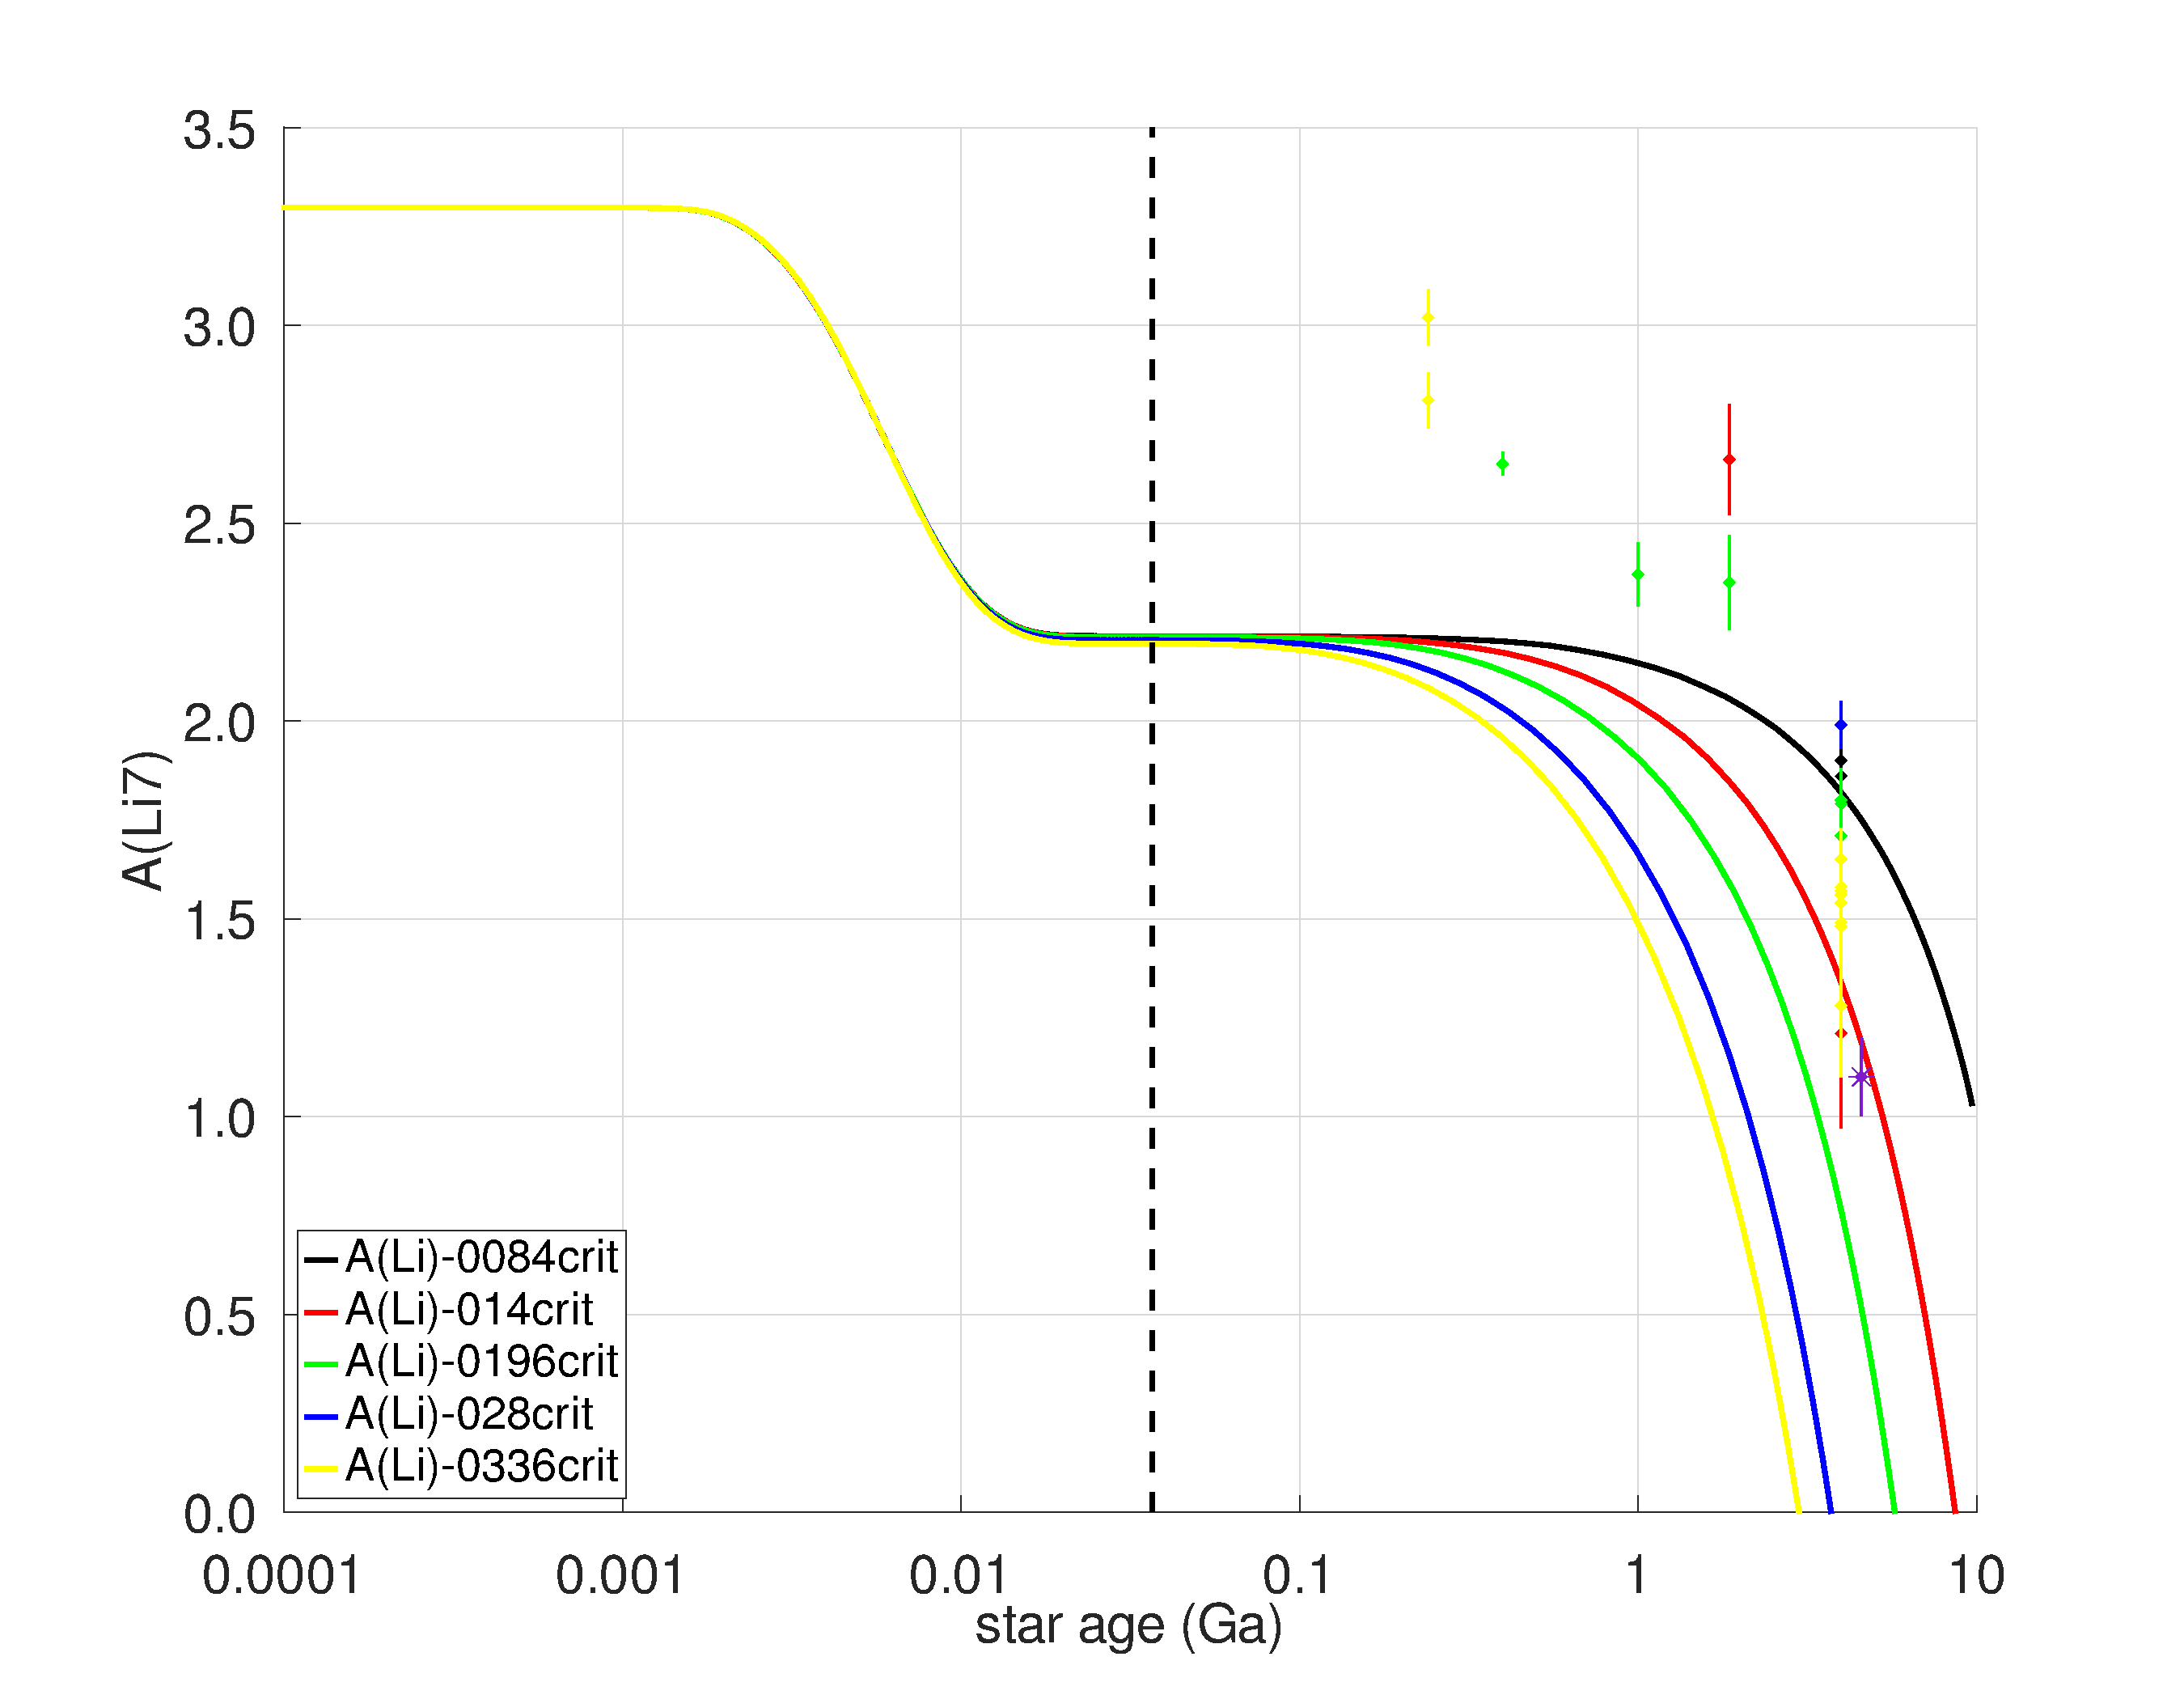
\includegraphics[width=0.7\textwidth]{img/paper2/li_var_vel_0_0g_0.pdf}
	\caption{Se representa la relación entre la abundancia superficial del isotope[7]{Li} y el isotope[1]{H} en función del tiempo para varios modelos de 1 $\msun$ sin campo magnético. El modelo de referencia, propuesto por \cite{Choi2016}, está representado por la línea negra continua. Los modelos adicionales con tasas de rotación iniciales que van de 0.0084 a 0.0336 se ilustran con las líneas restantes. Las abundancias superficiales de Li para el Sol actual, indicadas por una estrella púrpura, se basan en el estudio de \cite{Asplund2009}. La línea vertical discontinua corresponde a la Secuencia Principal de Edad Cero (ZAMS).}
	\label{fig:li_var_vel_0g_ii}
\end{figure}

\begin{figure}
	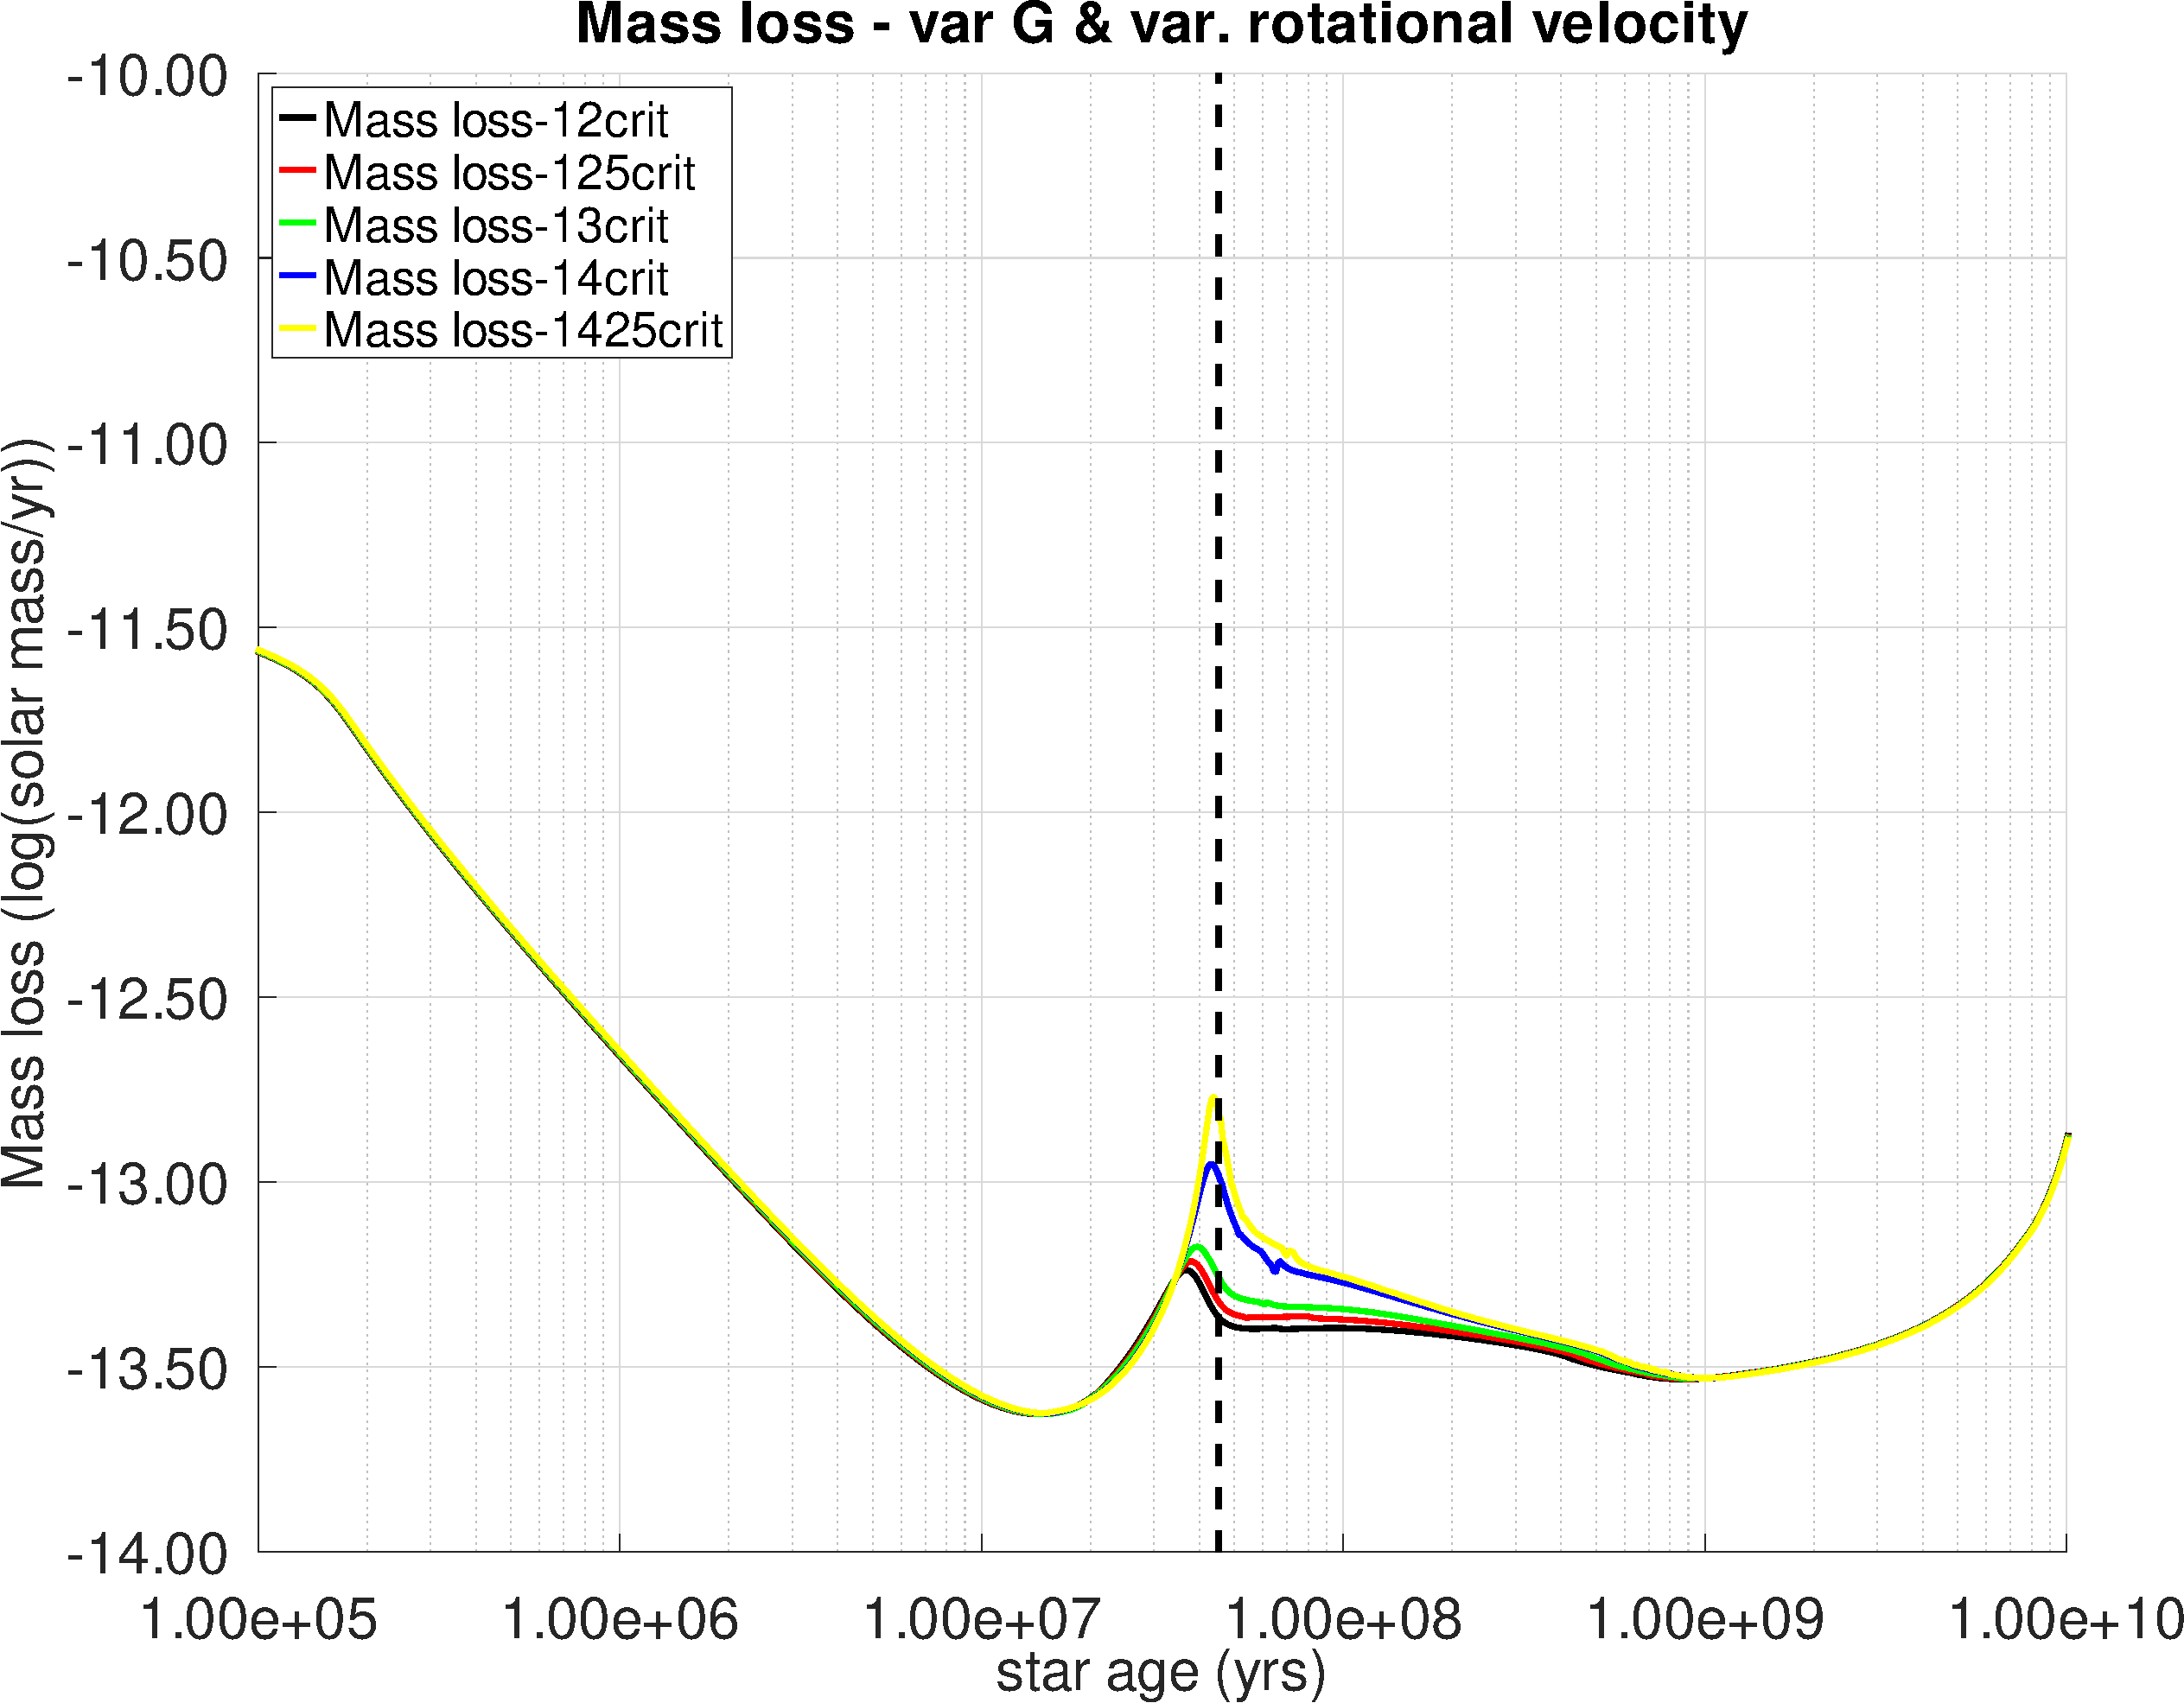
\includegraphics[width=0.7\textwidth]{img/paper2/mdot_var_vel_g3.pdf}
	\caption{Evolución de la pérdida de masa $\Dot{M}$ en función del tiempo para varios modelos de 1 $\msun$. Los modelos incluyen intensidad de campo magnético variable y rotación inicial con $\omegaini$ entre 0.12 y 0.1425. La línea vertical discontinua hace referencia a la ZAMS.}
	\label{fig:mdot_var_vel_g3}
\end{figure}


\begin{figure}
	\centering
	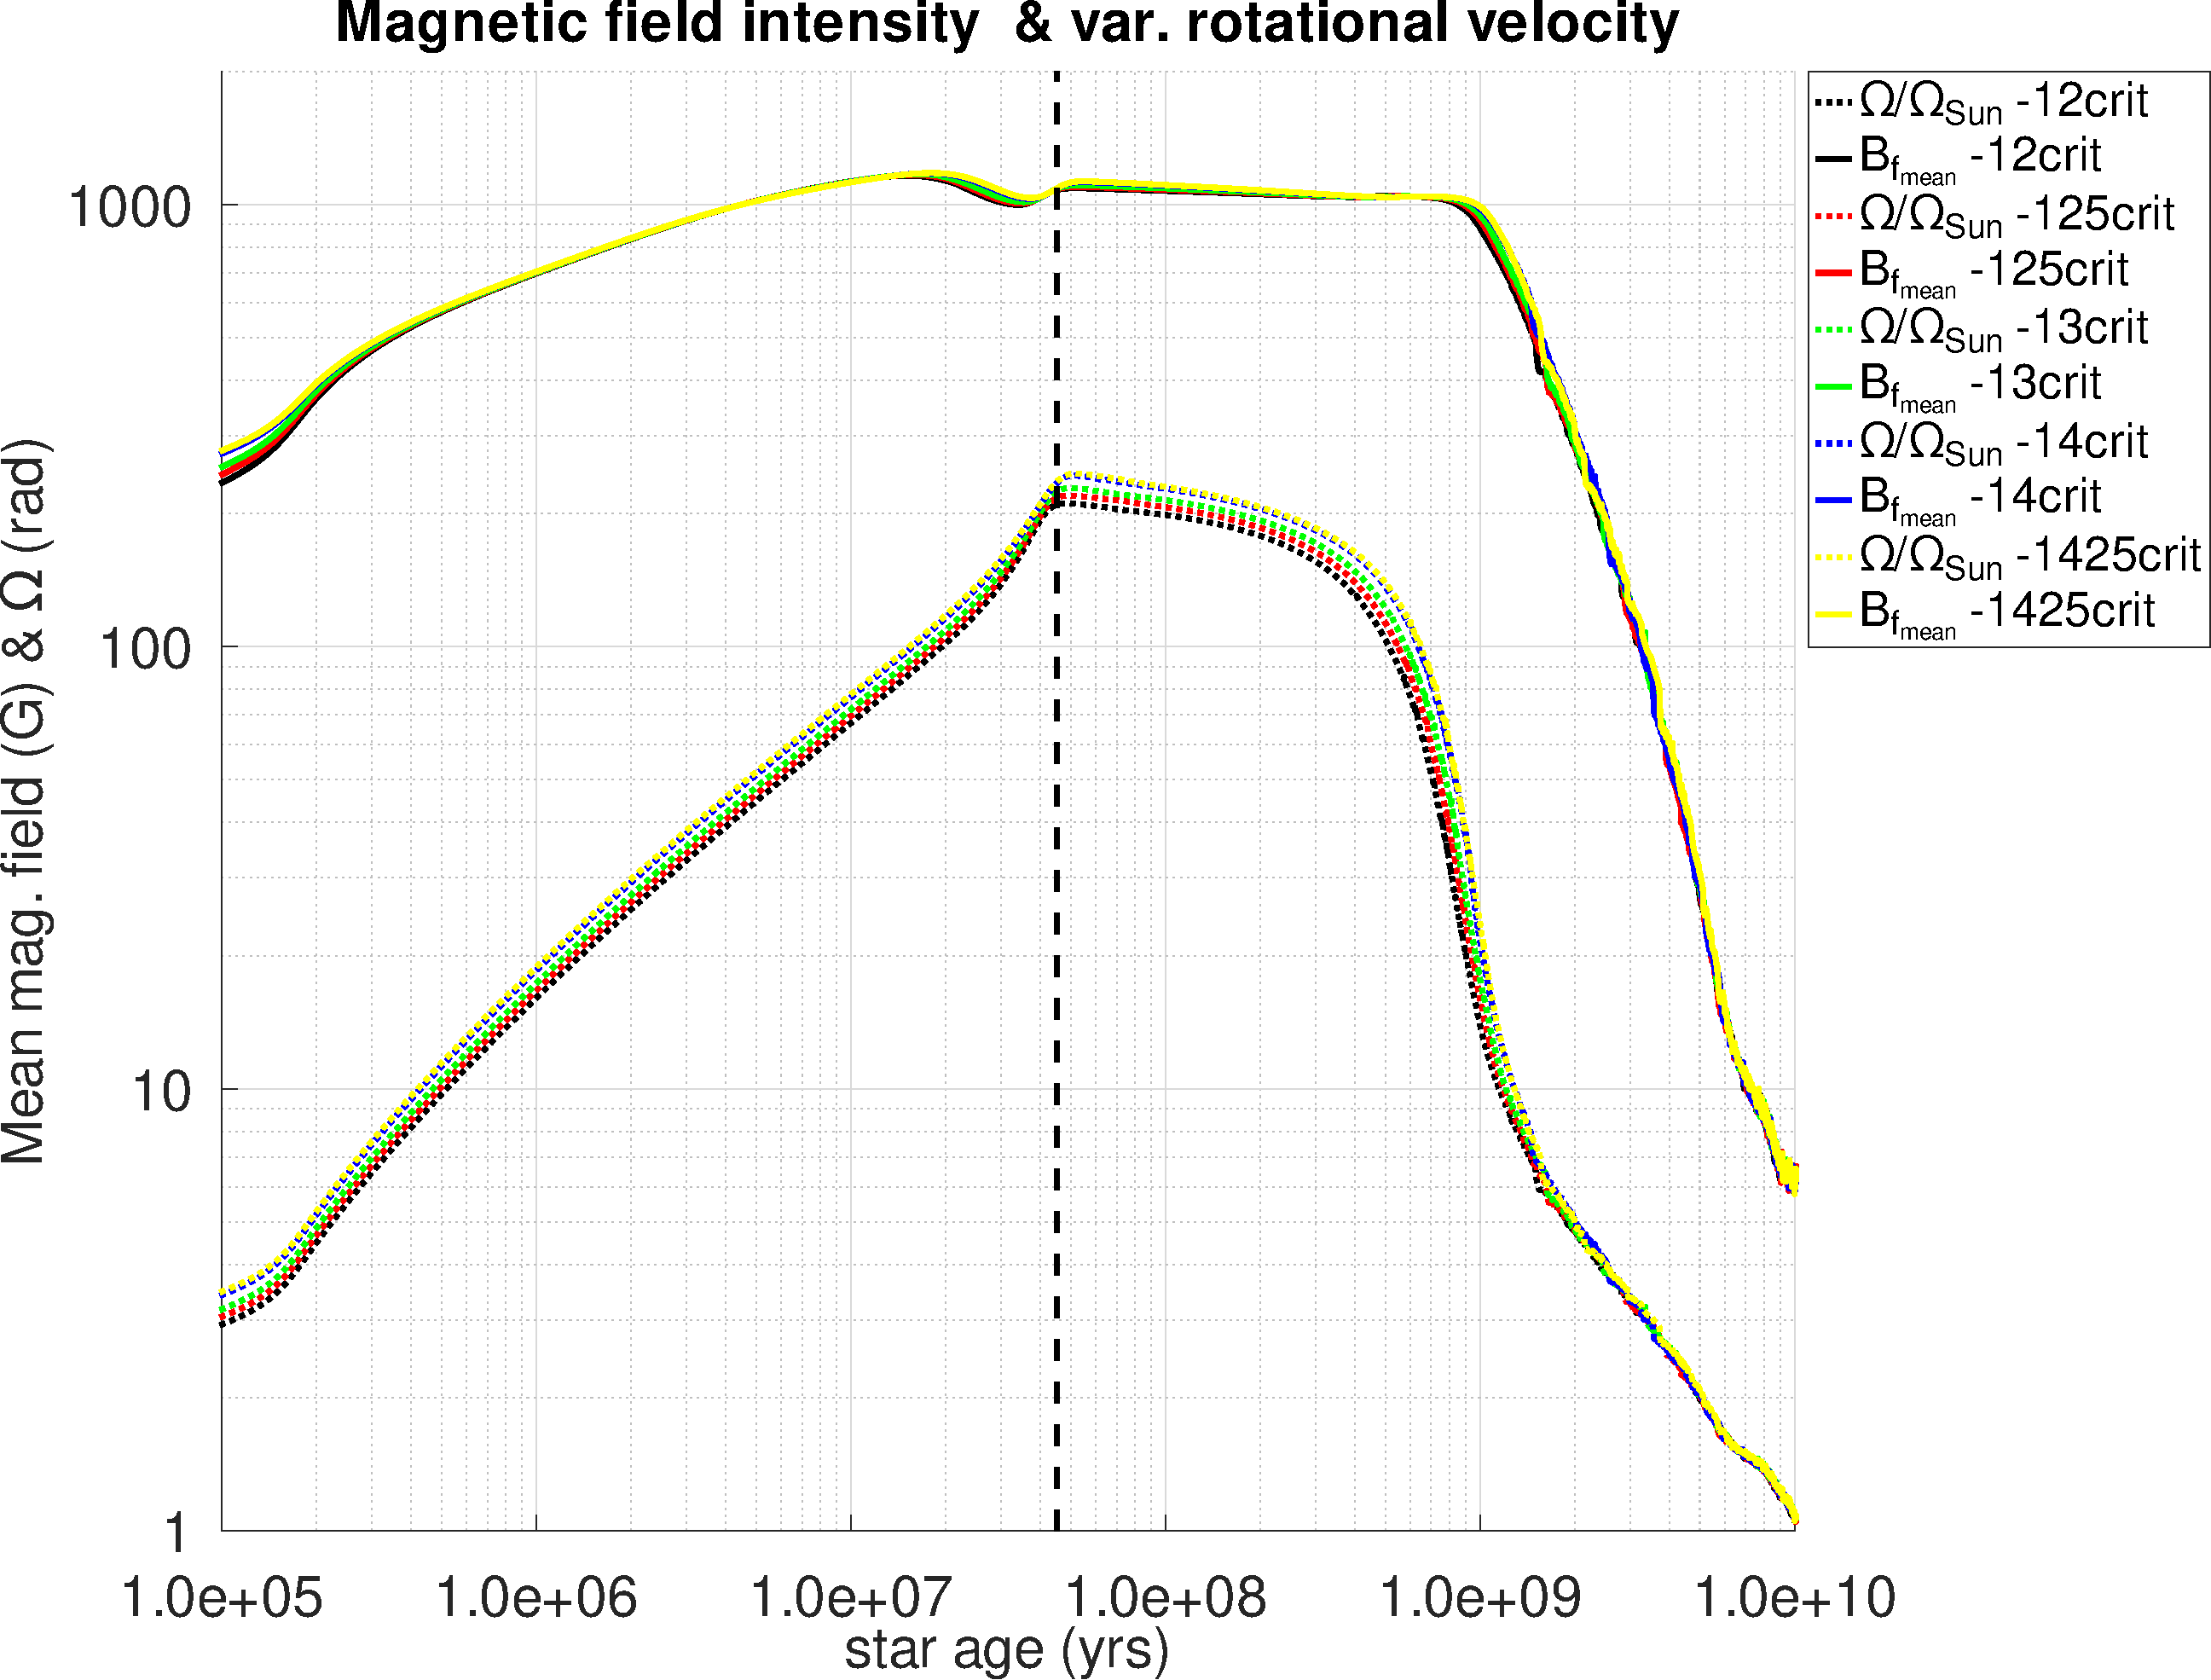
\includegraphics[width=0.7\textwidth]{img/paper2/mag_field_var_vel_g3.pdf}
	\caption{La evolución de la intensidad del campo magnético, en función del tiempo y $\omegaini$ para varios modelos de 1 $\msun$. Los modelos incluyen una rotación inicial con $\omegaini$ entre 0.12 y 0.1425. Las líneas continuas representan la intensidad del campo magnético, mientras que las líneas de puntos representan la evolución angular de la estrella. La línea vertical discontinua hace referencia a la ZAMS.}
	\label{fig:mag_field_var_vel_g3}
\end{figure}

En la Figura \ref{fig:rot_vel_var_vel_var_g3} se representan los perfiles de rotación de las estrellas para la superficie y para el fondo de la envoltura convectiva. Muestra cómo la velocidad angular aumenta de valor a medida que la estrella disminuye de radio a lo largo del PMS. Durante esta etapa de su evolución, la estrella tiene una estructura casi convectiva, como puede verse en la figura \ref{fig:cz_var_vel_var_g3}. A medida que se acerca a una edad de $\approx 10^6$ años, la zona convectiva de la estrella comienza a reducir su tamaño y el núcleo de la estrella alcanza las condiciones de temperatura, presión y densidad necesarias para desarrollar un núcleo radiativo. A su vez, la diferencia en las velocidades angulares de los distintos modelos se hace más evidente, siendo mayor en aquellos que fueron inicializados con una velocidad angular inicial más alta. Este hecho implica que la pérdida de masa también es mayor en aquellas estrellas que rotan más rápido. Como hemos descrito anteriormente, una mayor pérdida de masa implica también una mayor pérdida de momento angular. Los efectos combinados de los aumentos de la temperatura efectiva, la velocidad angular y la pérdida de masa hacen que la intensidad del campo magnético alcance su máximo en la fase de aproximación de la ZAMS (véase la figura \ref{fig:mag_field_var_vel_g3}). Observamos que los modelos con menor velocidad angular generalmente terminan exhibiendo valores más altos para la abundancia de Li en la superficie (ver Figuras~ \ref{fig:li_var_vel_var_g_3}, \ref{fig:grid_li_var_vel} \& \ref{fig:grid_li_var_g}).\par

Para los modelos en los que obtenemos valores de A(Li) en sintonía con los del Sol ($\omegaini$ = 0.14 y 0.1425), tenemos en cambio medidas para el $\Omega$ y $B$ que no están en sintonía con los solares respectivos. La velocidad de rotación de la superficie del Sol es de 2km/s con un error mínimo de 3m/s, y la intensidad media del campo magnético es de 1G. Para la simulación con $\omegaini$=0.1425, obtenemos una velocidad de rotación en el ecuador de 4.72 km/s. Aunque se trata de una medida del mismo orden de magnitud, representa una desviación del 235\%. Para la intensidad media del campo magnético tenemos 36.9G, muy lejos del valor de referencia.\par

Como se describe en la sección \ref{mod_mb}, la rutina MB, que se activa cuando la estrella desarrolla un núcleo radiativo y una zona convectiva sobre él (ver Figura \ref{fig:mb_act_var_vel_g3}), distribuyó la cantidad total de LMA calculada según la Ec.~\ref{eq:k_jdot} entre las distintas capas que componían la CZ. En la Figura \ref{fig:cz_var_vel_var_g3} podemos observar la evolución de la CZ más externa normalizada con respecto al radio de la estrella para varios modelos de 1 $\msun$. De acuerdo con los modelos establecidos de evolución estelar, en una estrella de tipo solar la CZ cubre prácticamente en su totalidad gran parte del PMS. A partir de la ZAMS, su tamaño comienza a disminuir gradualmente en una primera fase y luego se hace más pronunciado en torno a los $4.0x10^8$ años de edad. Como puede verse en la figura \ref{fig:rot_vel_var_vel_var_g3}, la estrella, tras alcanzar su velocidad angular máxima al pasar por la ZAMS, comienza a desacelerar debido al frenado magnético.\par

Es la presencia del MB la que impide que la estrella siga aumentando su velocidad angular. De este modo, la destrucción del Li se ve atenuada por una menor velocidad de rotación. Los modelos comienzan a desacelerarse gradualmente una vez superada la ZAMS y durante el periodo inicial de su estancia en la EM. La intensidad del campo magnético se mantiene cerca de su máximo, disminuye ligeramente y luego se reduce de forma más acusada. Su comportamiento refleja el de la evolución de la velocidad angular, consecuencia de los efectos de la MB. El proceso de desaceleración continúa progresivamente hasta que, en torno a la edad actual del Sol, se obtienen valores de velocidad angular muy similares a los del Sol. La desaceleración conduce a un menor efecto de las fuerzas centrífugas, lo que permite una contracción del radio de la estrella y, por tanto, un menor tamaño del CZ. Además, una menor velocidad angular tiene un efecto sobre la intensidad del campo magnético, como puede verse en la Figura \ref{fig:mag_field_var_vel_g3}. El acoplamiento entre la velocidad angular, la intensidad del campo magnético y el radio de la estrella es evidente y coherente.\par

\begin{figure}
	\centering
	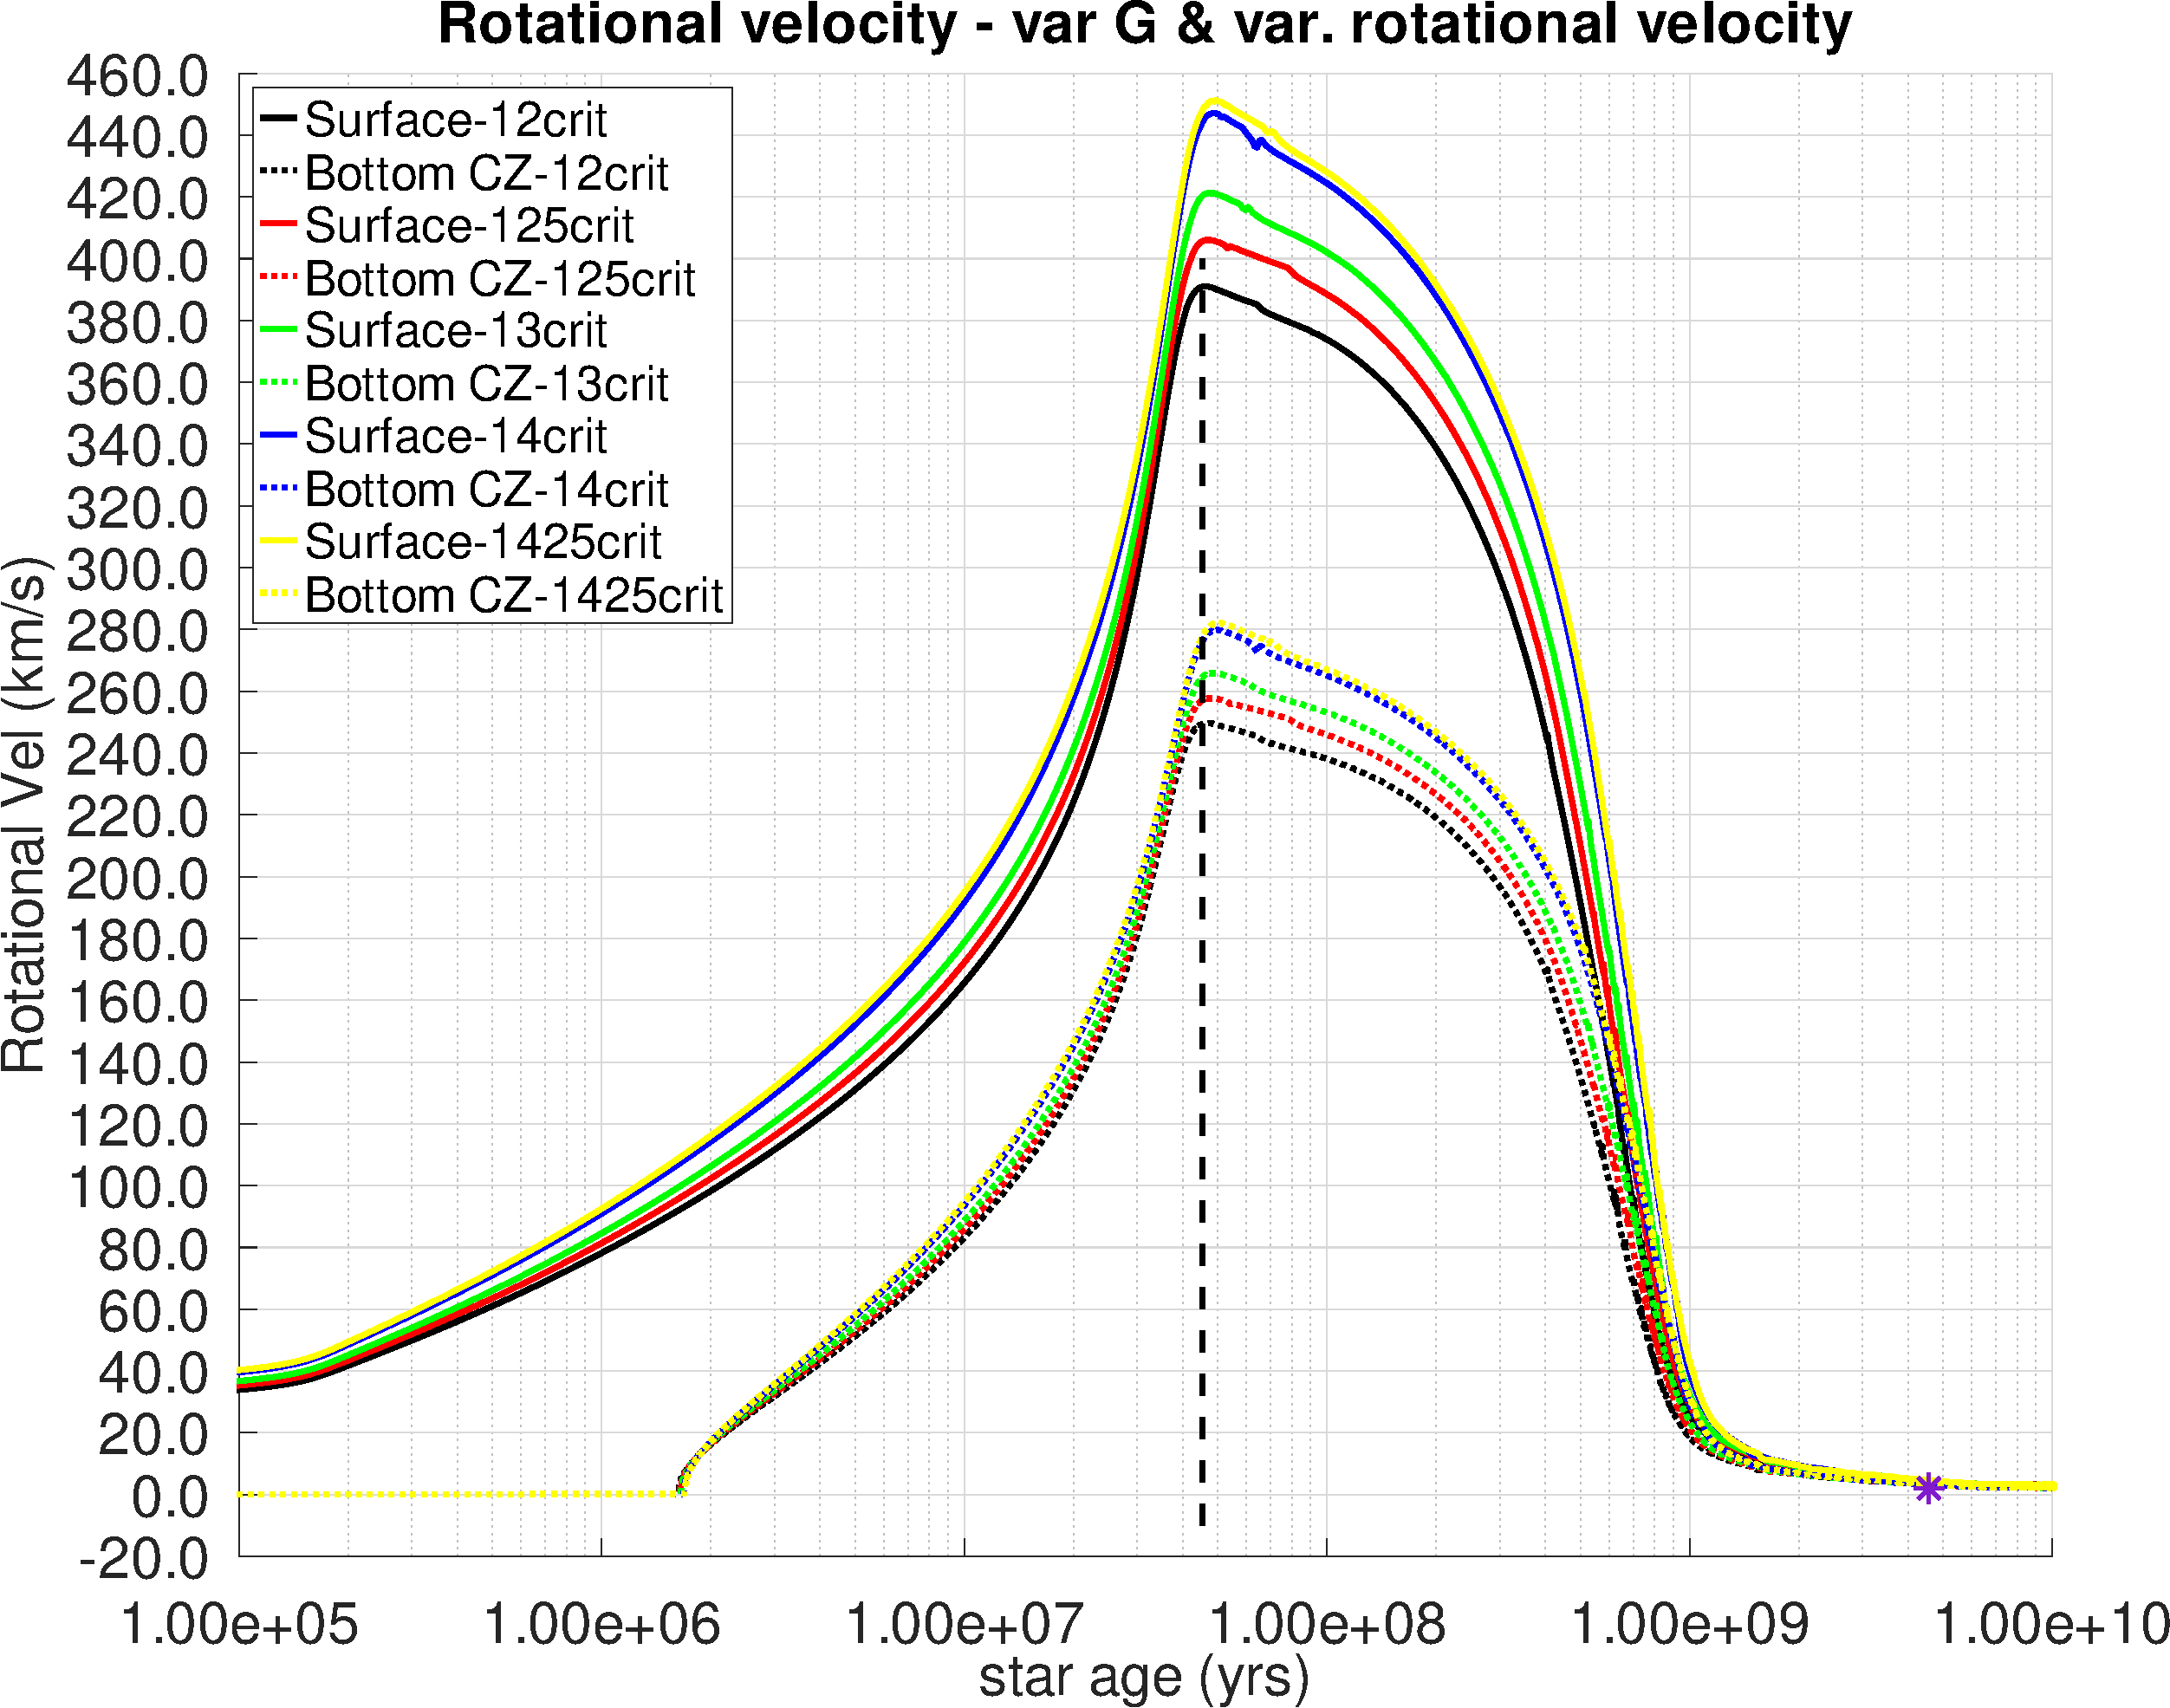
\includegraphics[width=0.7\textwidth]{img/paper2/rot_vel_var_vel_var_g3.pdf}
	\caption{La evolución de la velocidad de rotación de la superficie, en función del tiempo para varios modelos de 1 $\msun$. Los modelos incluyen un campo magnético de intensidad variable, rotación inicial con $\omegaini$ entre 0.12 y 0.1425, respectivamente y MB. La estrella púrpura es la velocidad angular superficial para el Sol actual \cite{Gill2012}. La línea vertical discontinua hace referencia a la ZAMS.}
	\label{fig:rot_vel_var_vel_var_g3}
\end{figure}

\begin{figure}
	\centering
	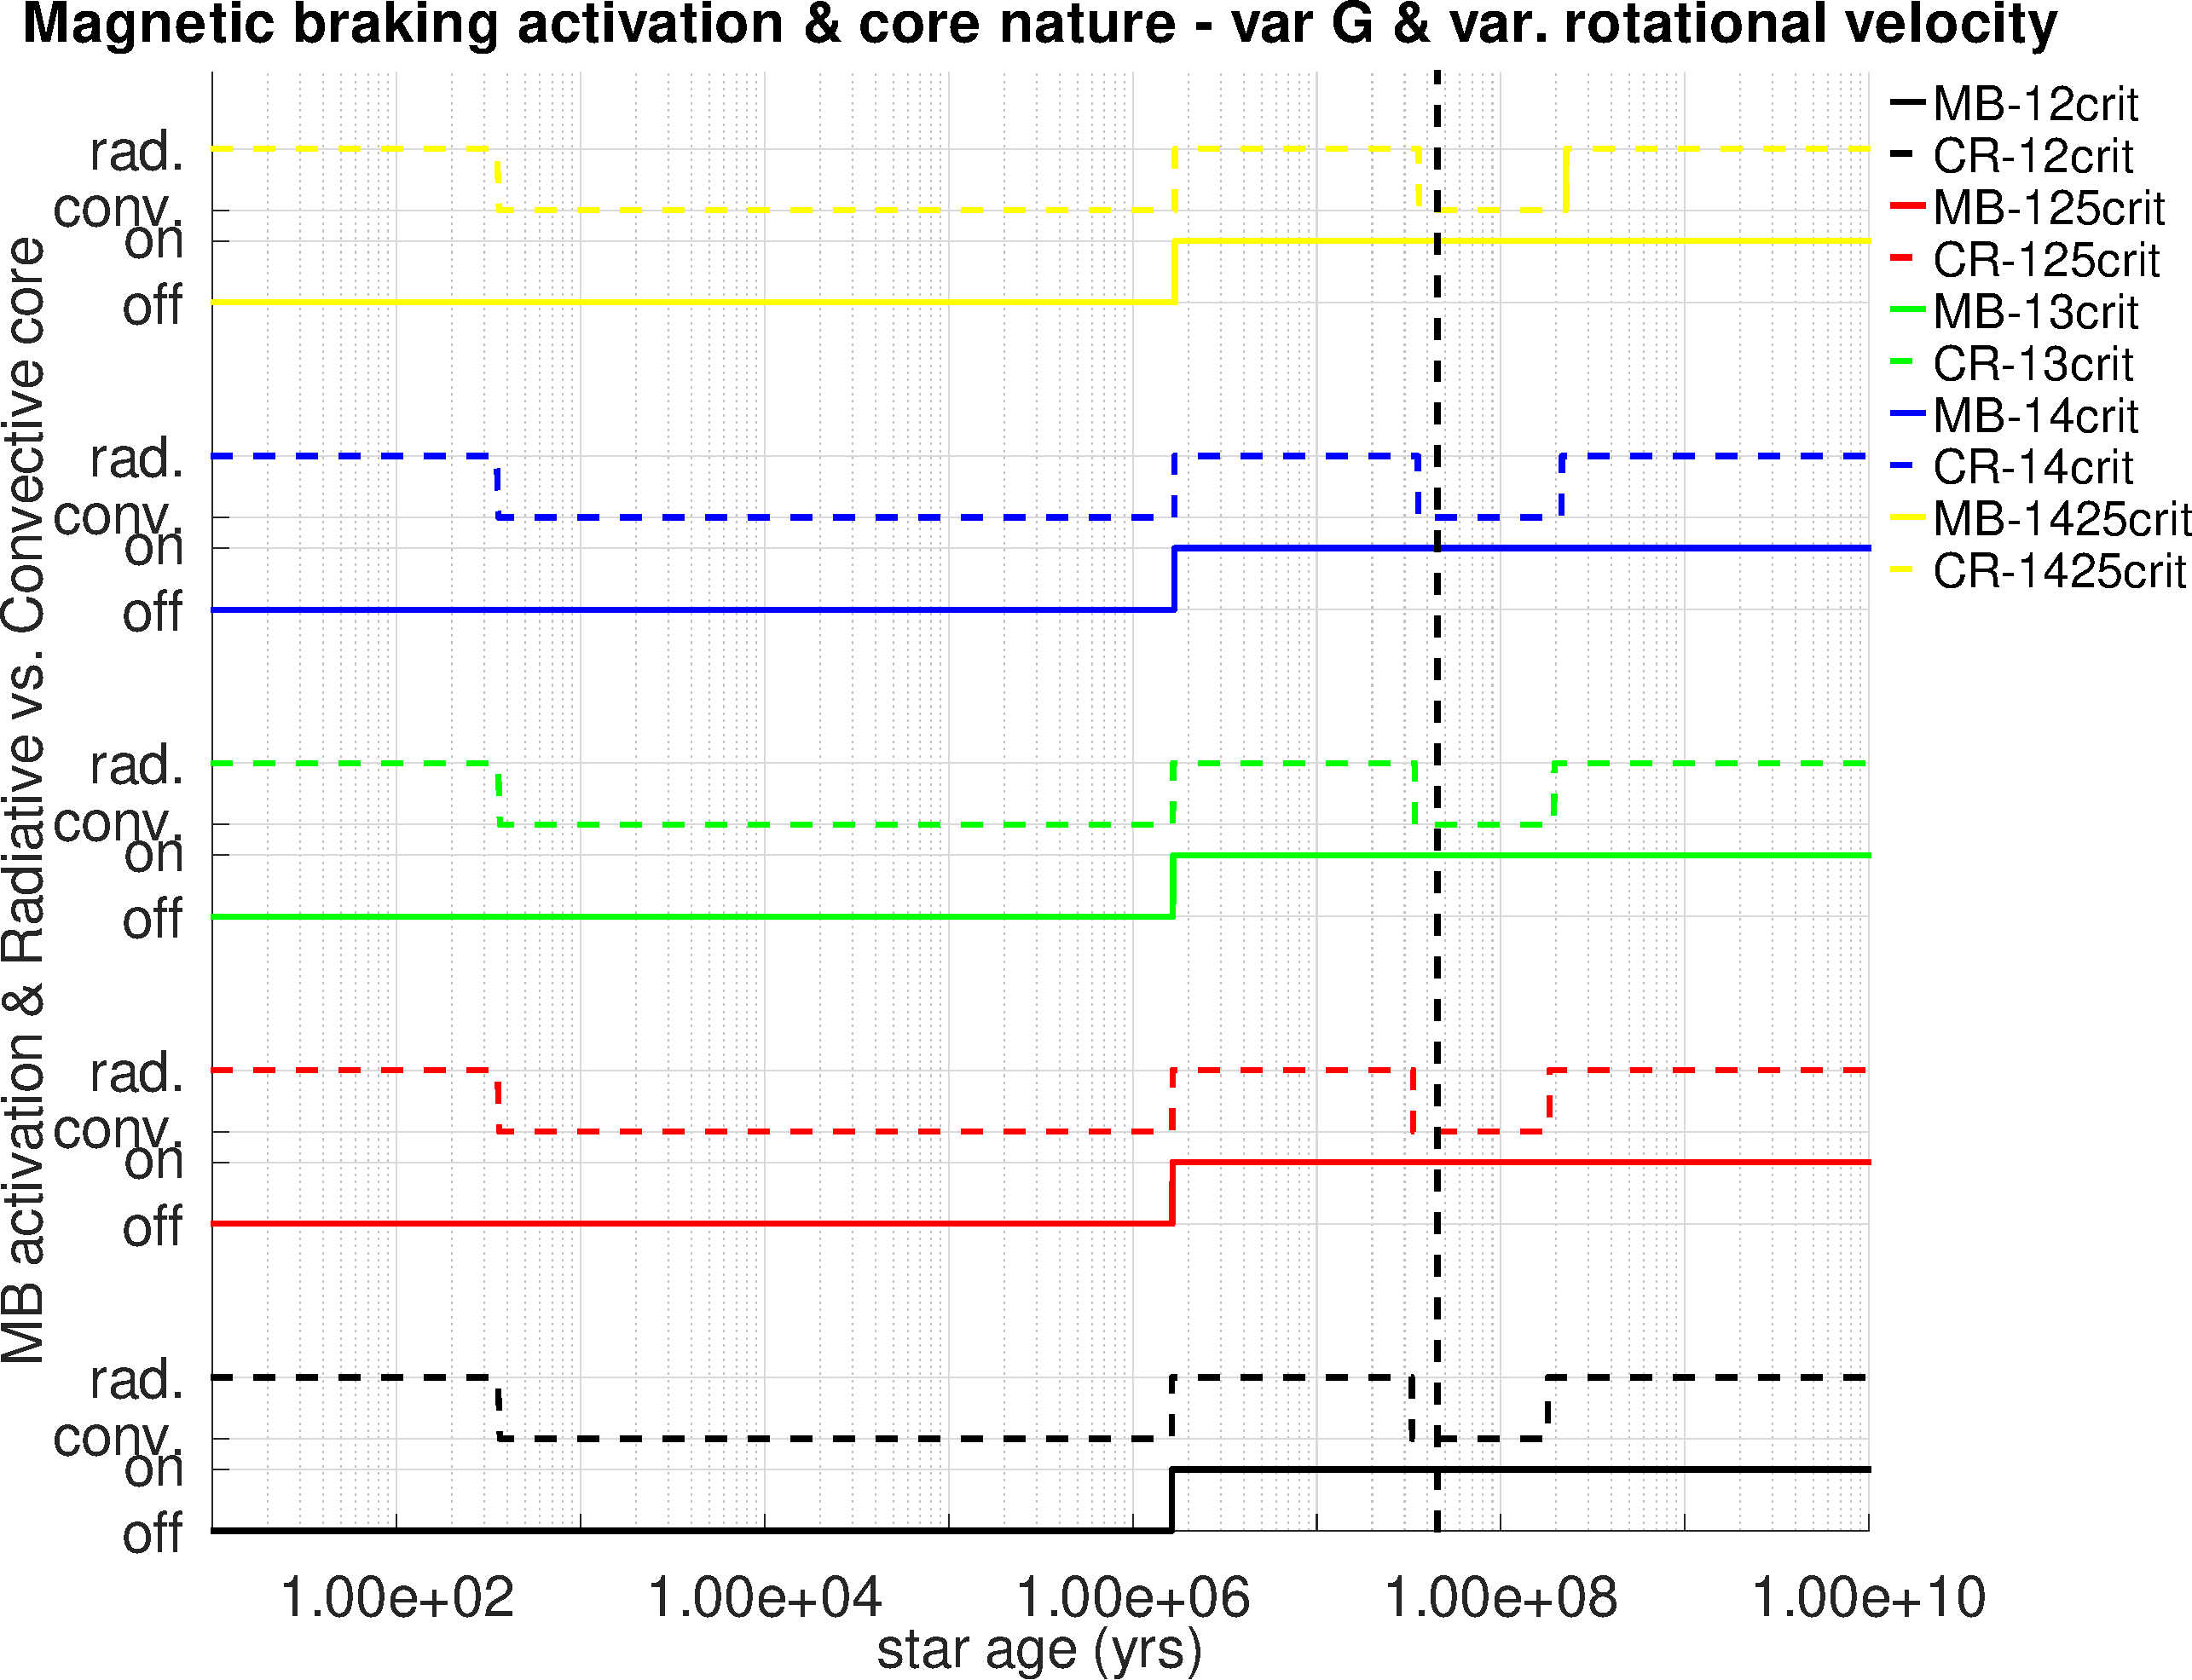
\includegraphics[width=0.7\textwidth]{img/paper2/mb_act_var_vel_g3.pdf}
	\caption{La activación de la rutina de frenado magnético en función de la presencia de un núcleo radiativo. Las líneas continuas señalan la activación (on) y desactivación (off) de la rutina de frenado magnético. Las líneas horizontales discontinuas informan sobre la naturaleza del núcleo de la estrella: radiativo (rad) o convectivo (conv). Por decisión de implementación, una vez activada la rutina, permanece activada incluso si la naturaleza del núcleo de la estrella cambia a convectiva. La línea vertical discontinua hace referencia a la ZAMS.}
	\label{fig:mb_act_var_vel_g3}
\end{figure}

\begin{figure}
	\centering
	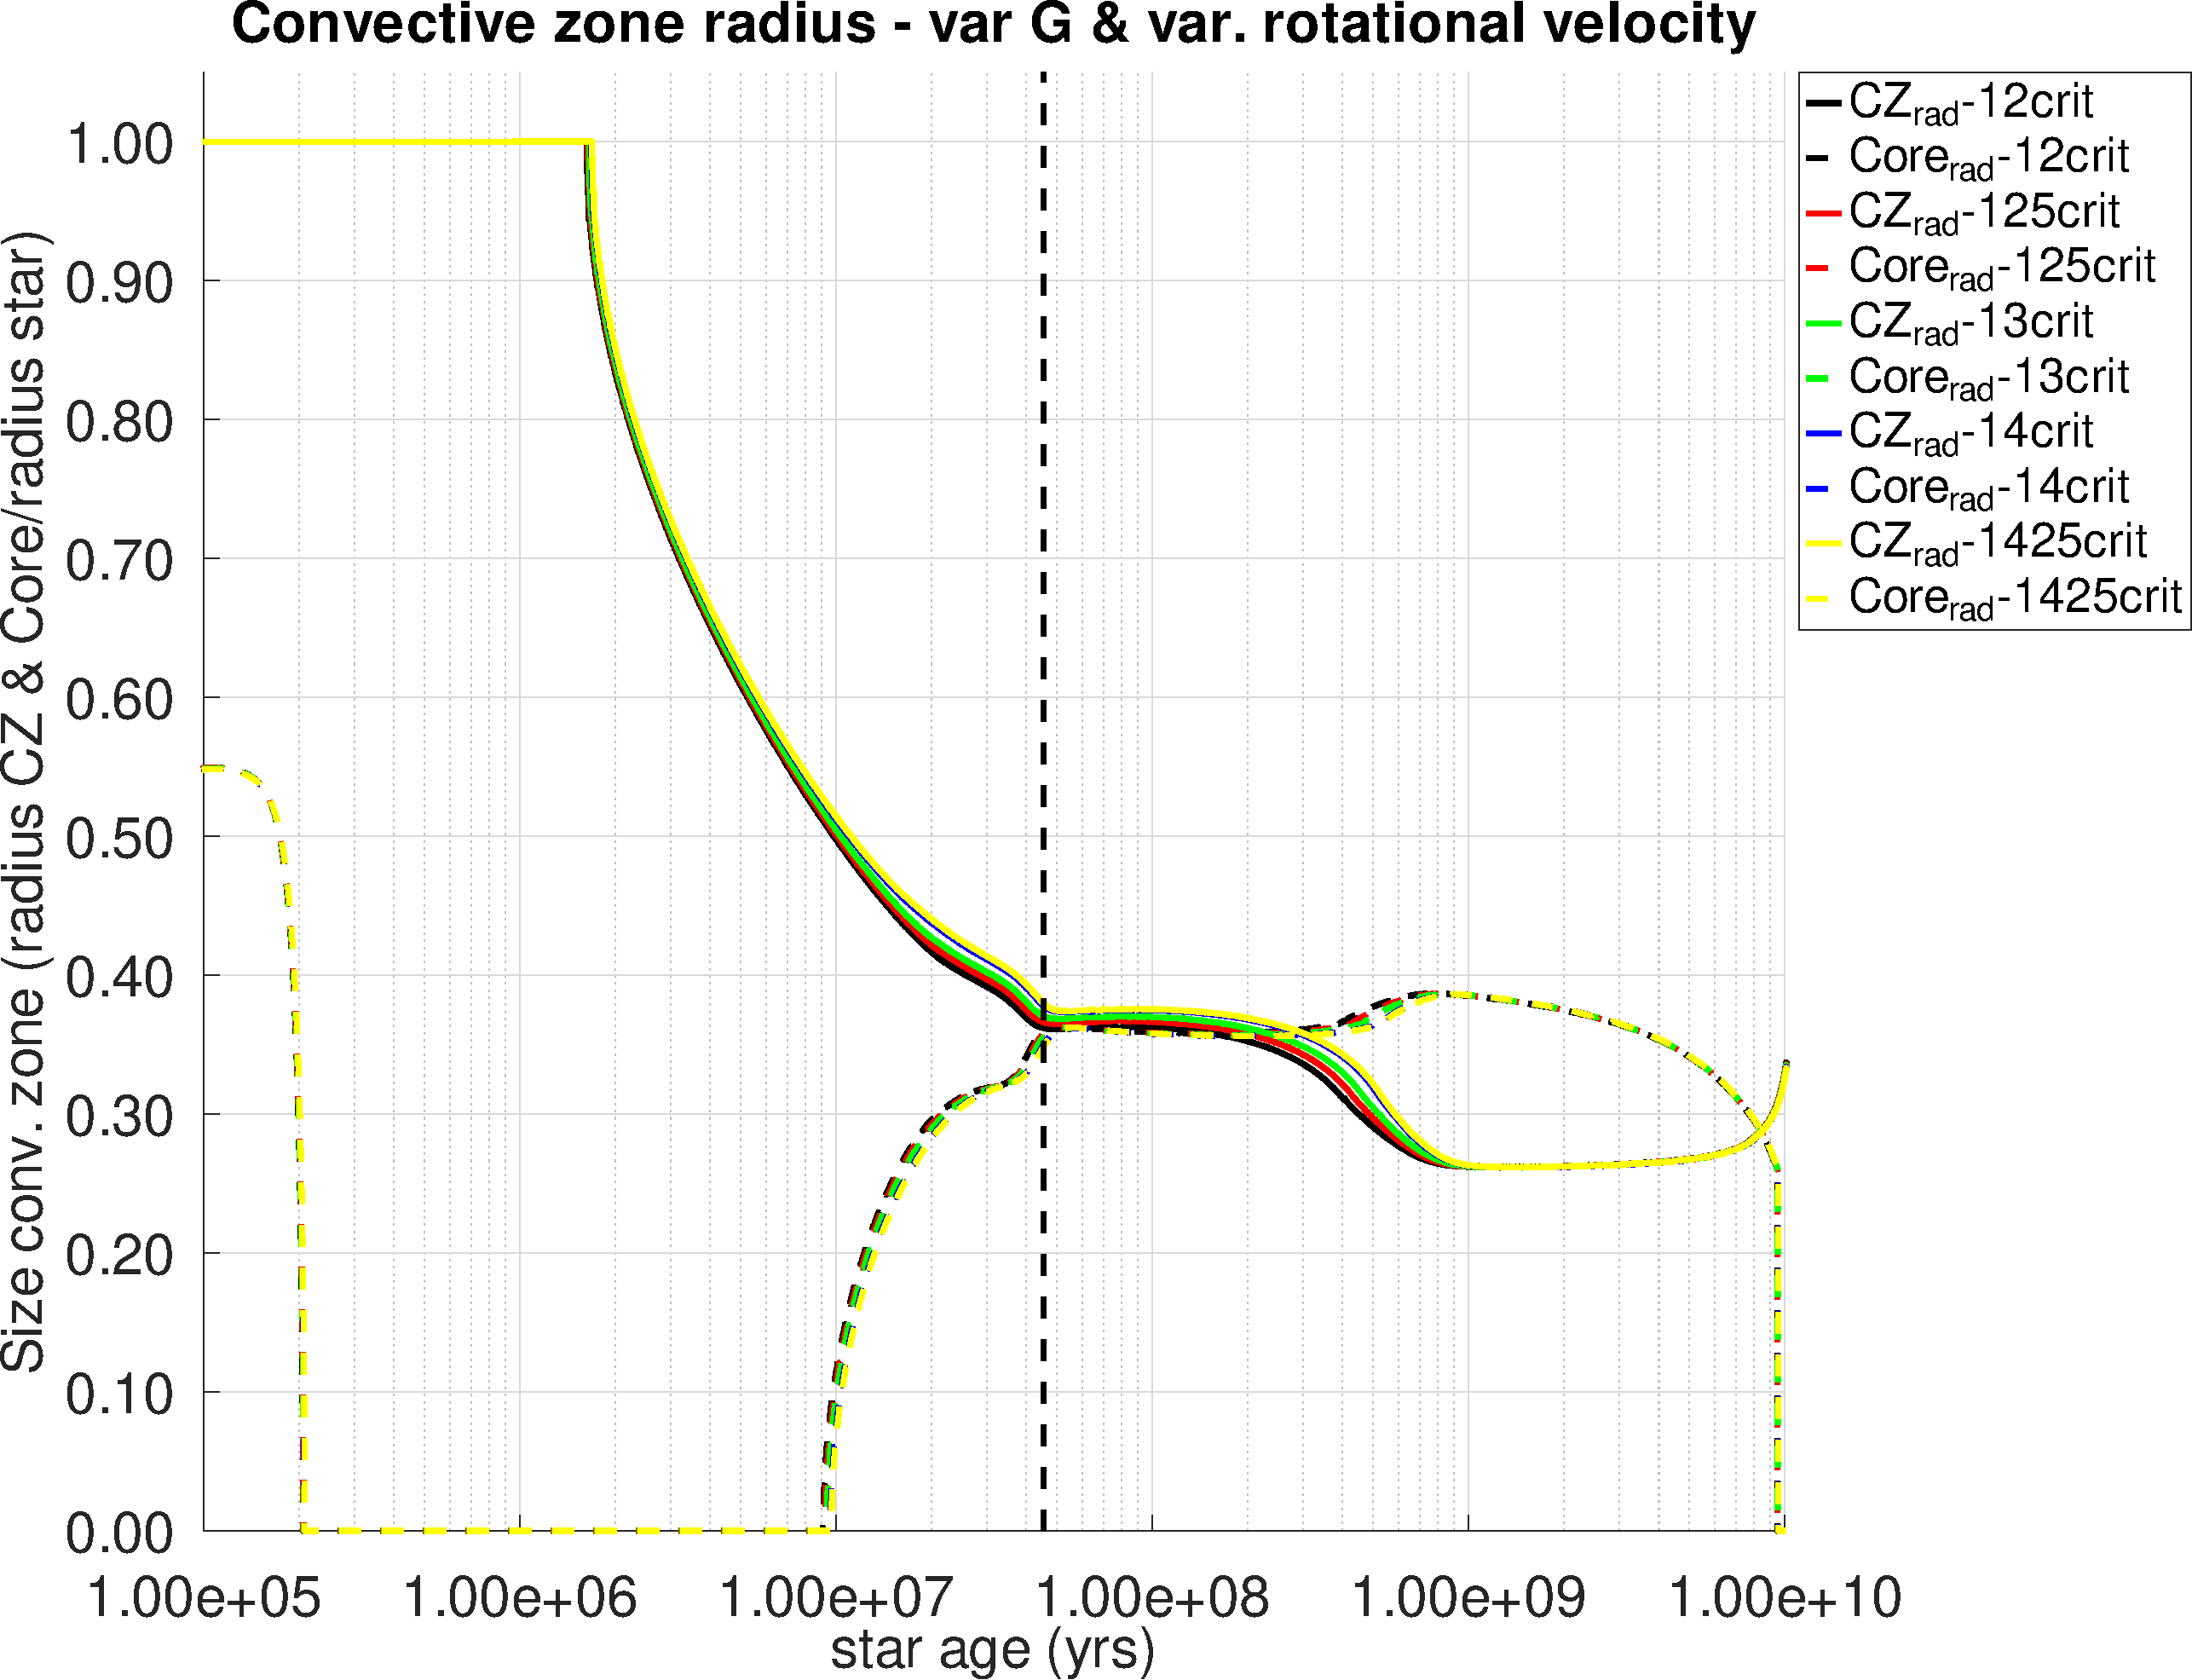
\includegraphics[width=0.7\textwidth]{img/paper2/cz_var_vel_var_g3.pdf}
	\caption{SUSTITUIR POR GRÁFICA MOSTRANDO SOLO LA CZ. Evolución del tamaño de la zona convectiva en función del tiempo para varios modelos de 1 $\msun$. El tamaño se expresa en términos de $\rsun$. Los modelos incluyen un campo magnético de intensidad variable, rotación inicial con $\omegaini$ entre 0.12 y 0.1425. La línea vertical discontinua hace referencia a la ZAMS.}
	\label{fig:cz_var_vel_var_g3}
\end{figure}


\subsection{Evolución del Li con MB de intensidad y $\amlt$ variables}
Los efectos de la rotación y el frenado magnético también pueden observarse en el diagrama H-R y en la evolución del $\amlt$. La inclusión de la rotación implica la aparición de fuerzas centrífugas que afectan tanto a la estructura de la estrella como a la composición química de los distintos estratos que la componen, así como a su temperatura y luminosidad. La rotación diferencial entre los límites del núcleo radiativo y las capas convectivas provoca efectos de mezcla en la denominada tacoclina. Los efectos de esta mezcla y de sus efectos hidrostáticos se rigen por la MLT, en la que el $\amlt$ desempeña un papel fundamental. Como ya se ha dicho, la MLT adolece de la arbitrariedad del valor de $\amlt$. La figura \ref{fig:alpha_mlt_var_vel_g3} muestra cómo evoluciona el parámetro $\amlt$ con el tiempo.\par 

\begin{figure}
	\centering
	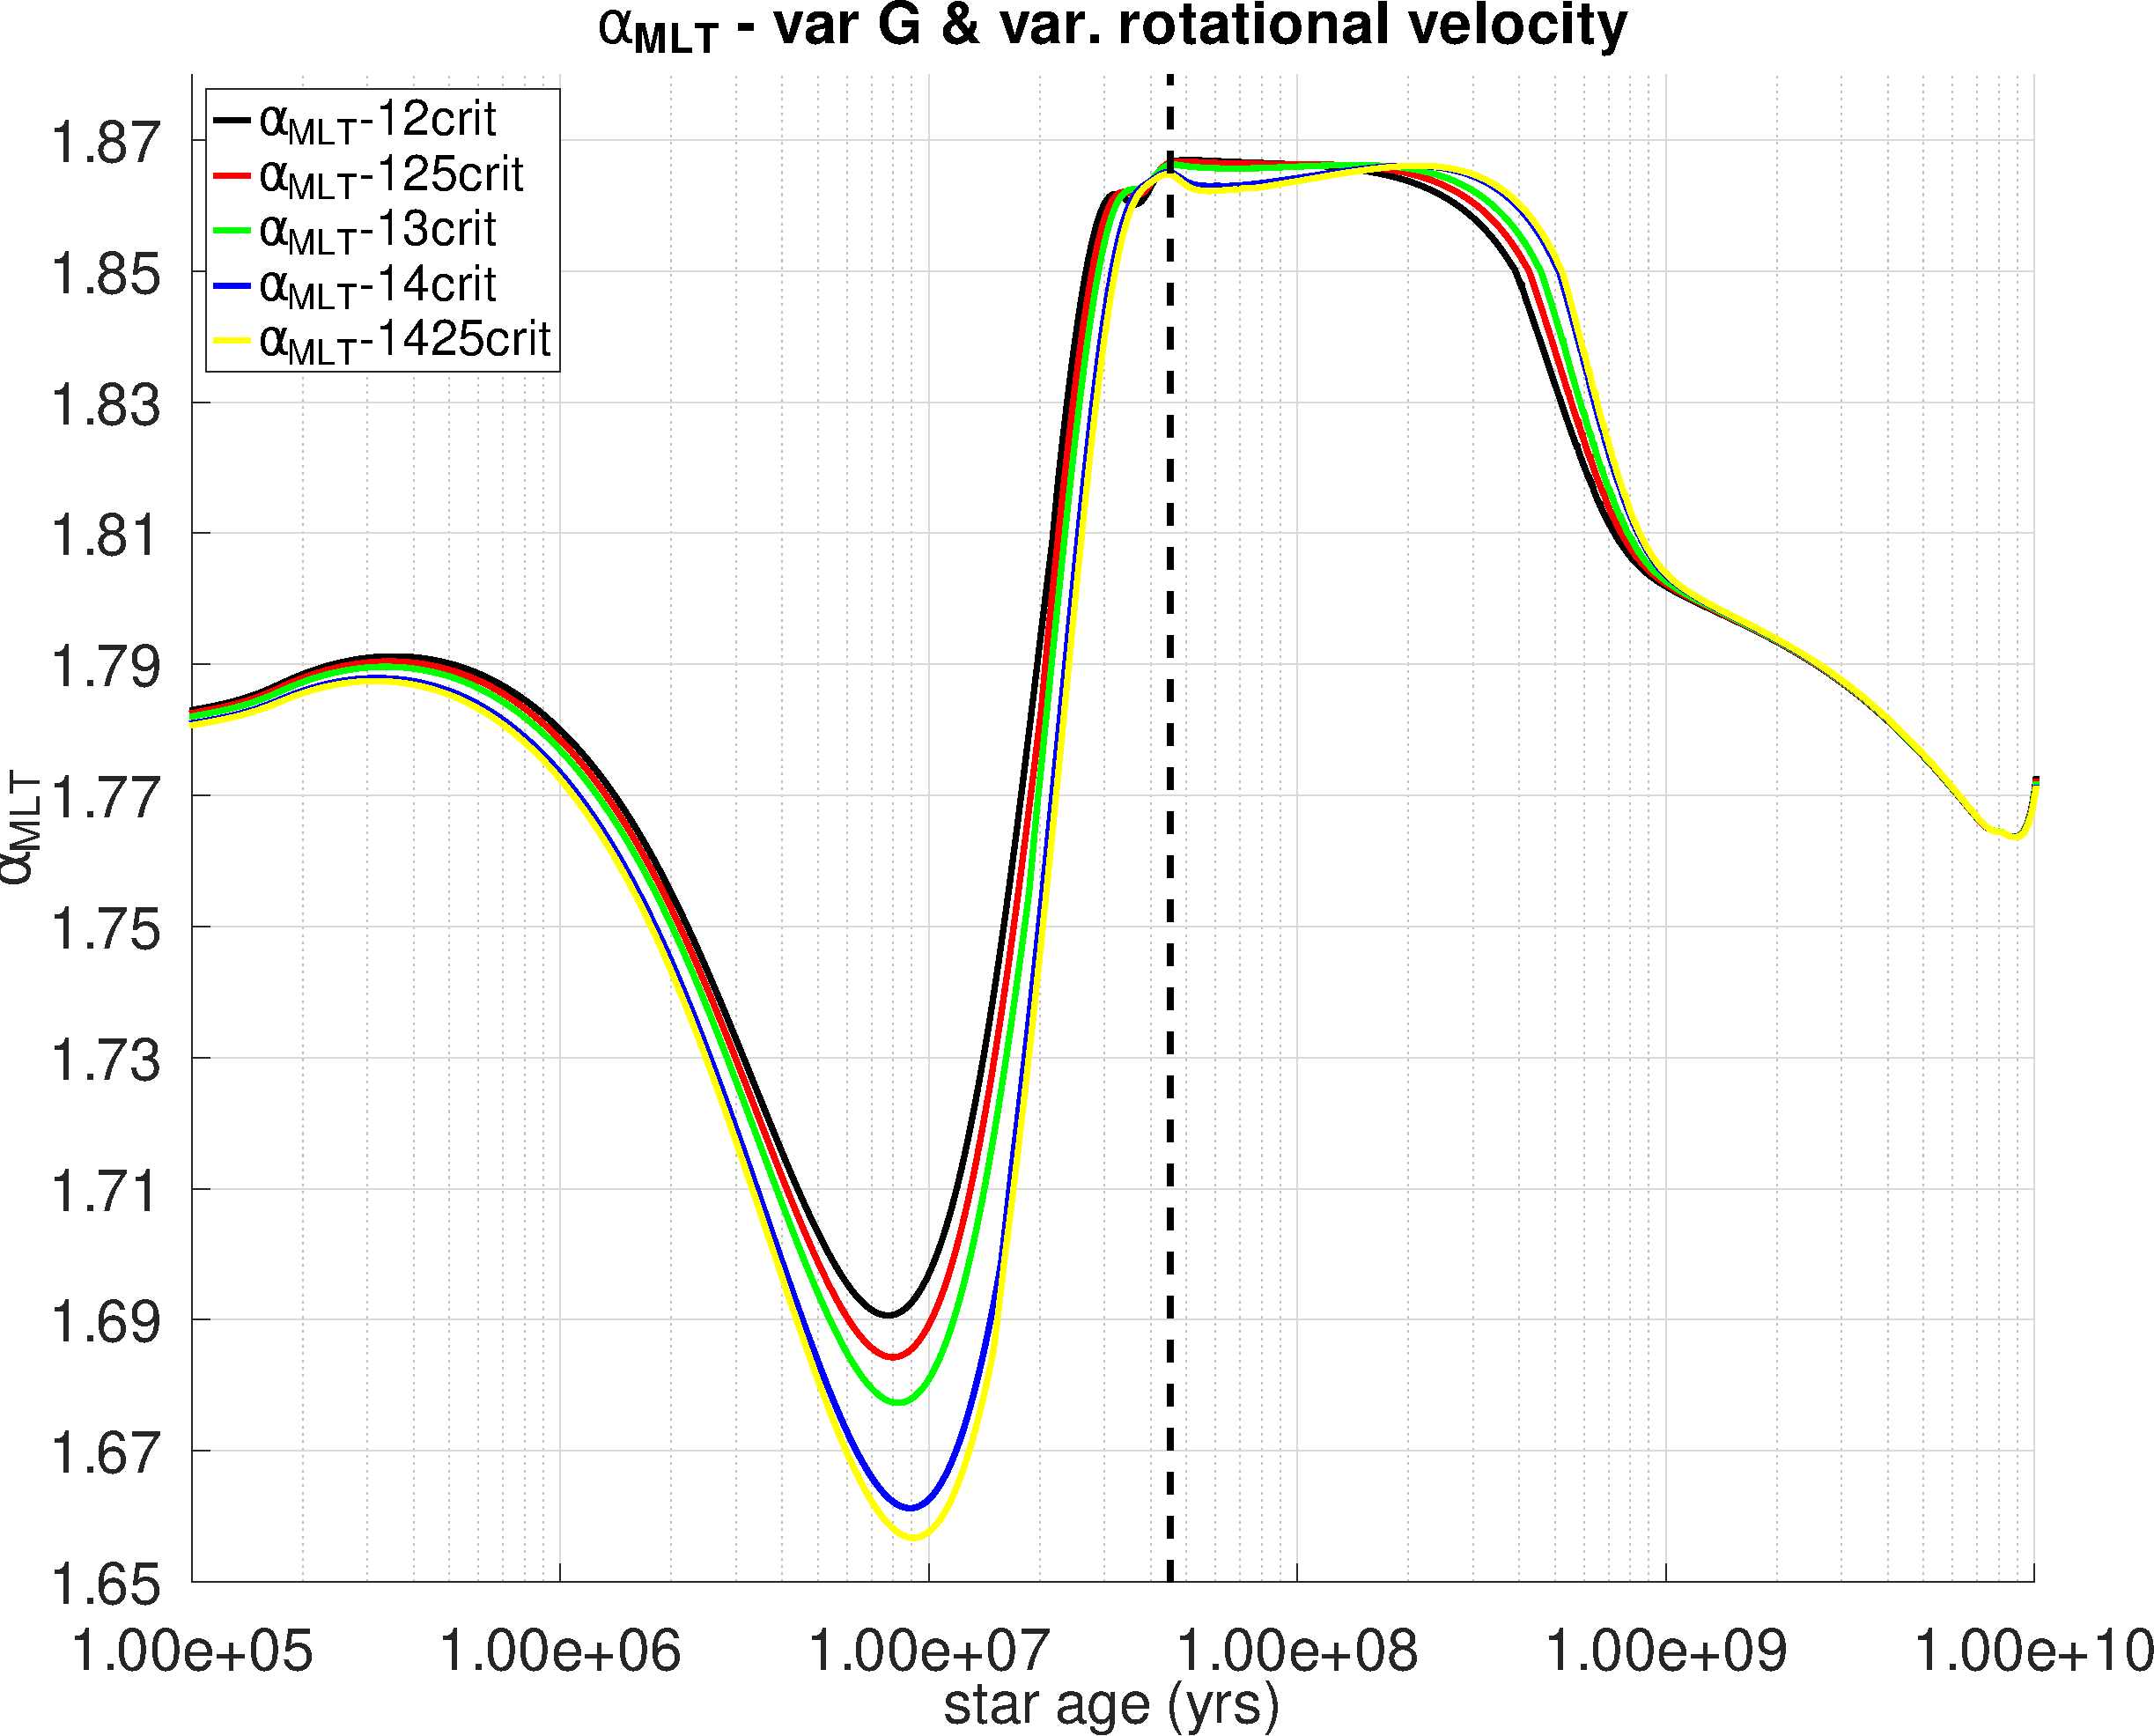
\includegraphics[width=0.7\textwidth]{img/paper2/alpha_mlt_var_vel_g3.pdf}
	\caption{La evolución de $\amlt$, en función del tiempo y $\omegaini$ para varios modelos de 1 $\msun$. Los modelos incluyen una rotación inicial con $\omegaini$ entre 0.12 y 0.1425. La línea vertical discontinua hace referencia a la ZAMS. La estrella púrpura y el rombo son los $\amlt$ dados por \cite{Sonoi2018} y \cite{Samadi2005}, respectivamente.}
	\label{fig:alpha_mlt_var_vel_g3}
\end{figure}

Además, estas mismas fuerzas centrífugas, acentuadas en estrellas con mayor velocidad angular, refuerzan también el oscurecimiento gravitatorio \cite[véase por ejemplo ][]{Eggenberger2012,Paxton2019,Gossage2021}. La fuerza centrífuga hace que la estrella desplace su masa hacia fuera con respecto al eje de rotación, siendo el efecto más pronunciado en las regiones ecuatoriales que en los polos. La consecuencia es que la presión ($\gsurf$) a la que está sometido el gas es menor en las primeras que en las segundas. Este efecto hace que las estrellas que rotan a gran velocidad aparezcan menos densas ($\rho$), menos luminosas ($L$) y, por tanto, con una temperatura efectiva ($\teff$) más baja a medida que se acercan a la ZAMS (véase la figura \ref{fig:hr_var_vel_var_g_z13}). Si comparamos el modelo no rotatorio (línea sólida negra en la Figura \ref{fig:hr_var_vel_0g}) con los rotatorios, podemos reconocer que al final del PMS, estos últimos alcanzan la ZAMS con un $\teff$ menor que los primeros. Esto también repercute en la evolución de $\amlt$ ya que, como se ha comentado anteriormente, en nuestro modelo su valor depende proporcionalmente de $\teff$ y $\gsurf$. Ambos parámetros son comparativamente menores en las estrellas que giran más rápido que en las que lo hacen más despacio. Como consecuencia $\amlt$ arroja un valor menor en su evolución temporal en aquellas fases en las que la estrella rota más rápido, siendo este efecto más acentuado en la aproximación ZAMS.\par

\begin{figure}
	\centering
	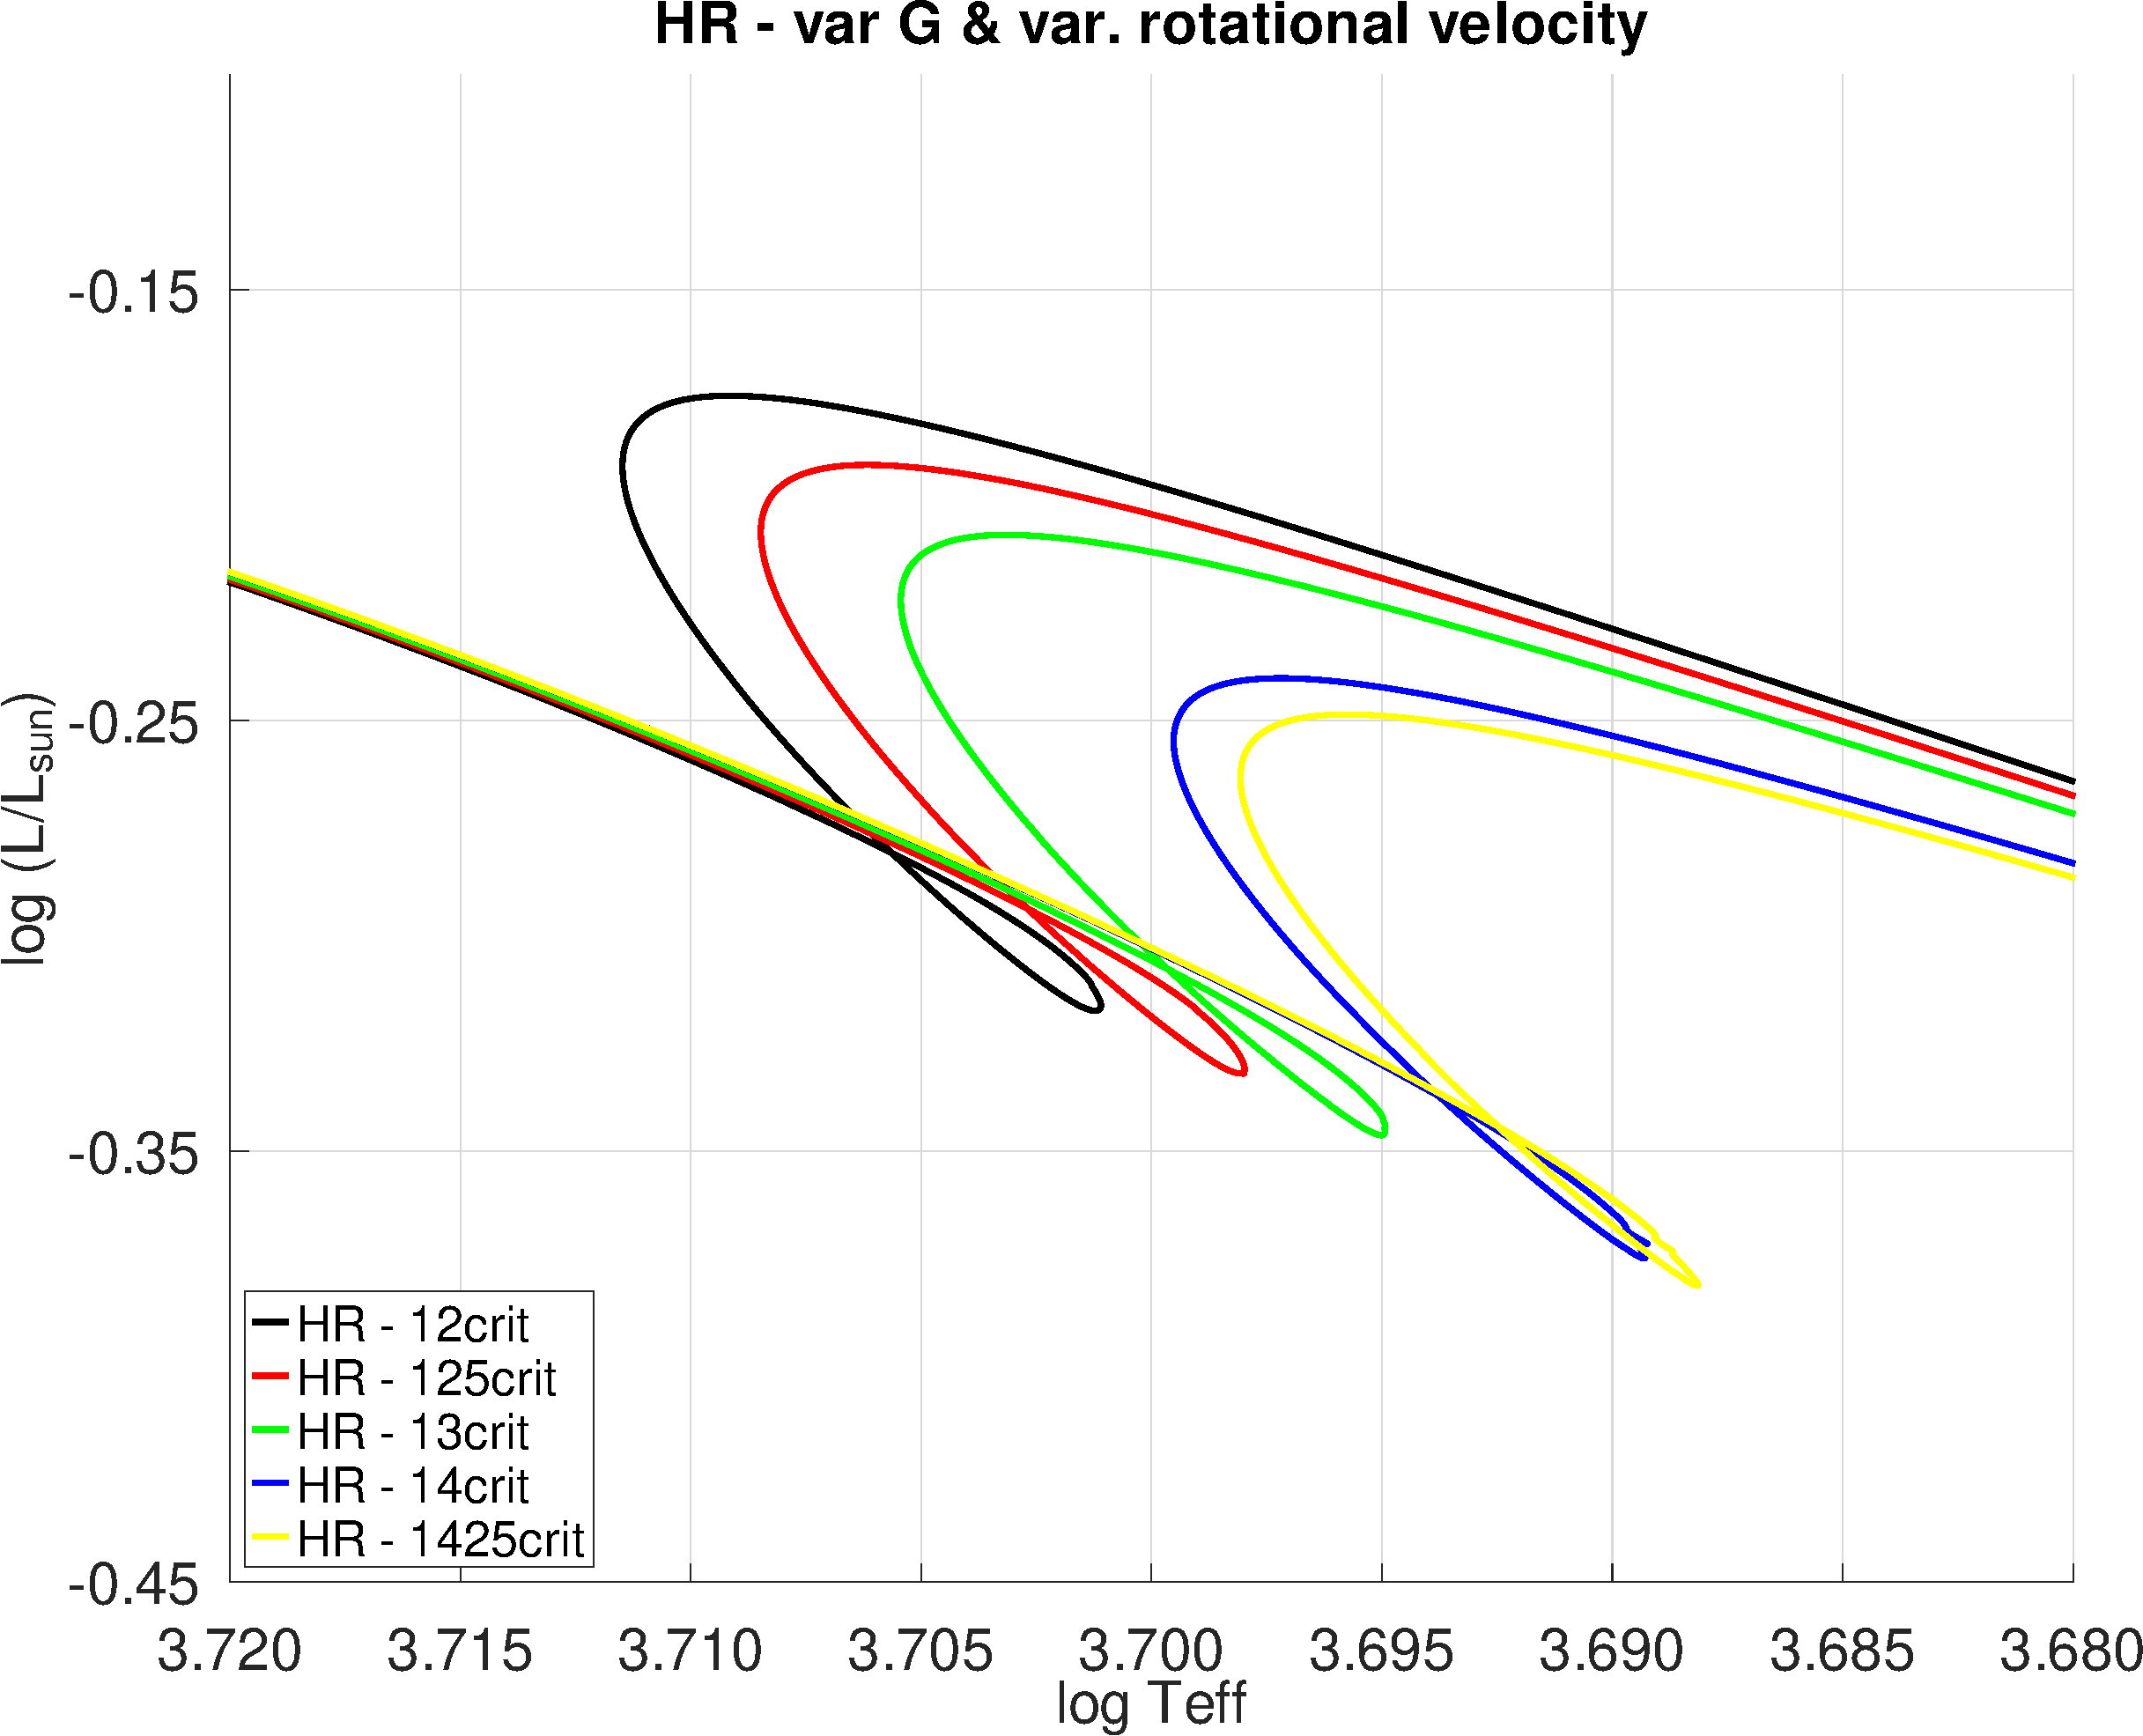
\includegraphics[width=0.7\textwidth]{img/paper2/hr_var_vel_var_g_z13.pdf}
	\caption{Un ejemplo de cuadrícula solar de 1$\msun$ de huellas evolutivas estelares que cubre un rango de velocidades angulares. Muestra en detalle los efectos combinados del oscurecimiento gravitatorio y el frenado magnético en las huellas evolutivas. Los modelos incluyen un campo magnético de intensidad variable, rotación inicial con $\omegaini$ entre 0.12 y 0.1425. La presencia de un campo magnético produce estrellas más calientes debido a la influencia del frenado magnético en la velocidad de rotación de la estrella.}
	\label{fig:hr_var_vel_var_g_z13}
\end{figure}

\begin{figure}
	\centering
	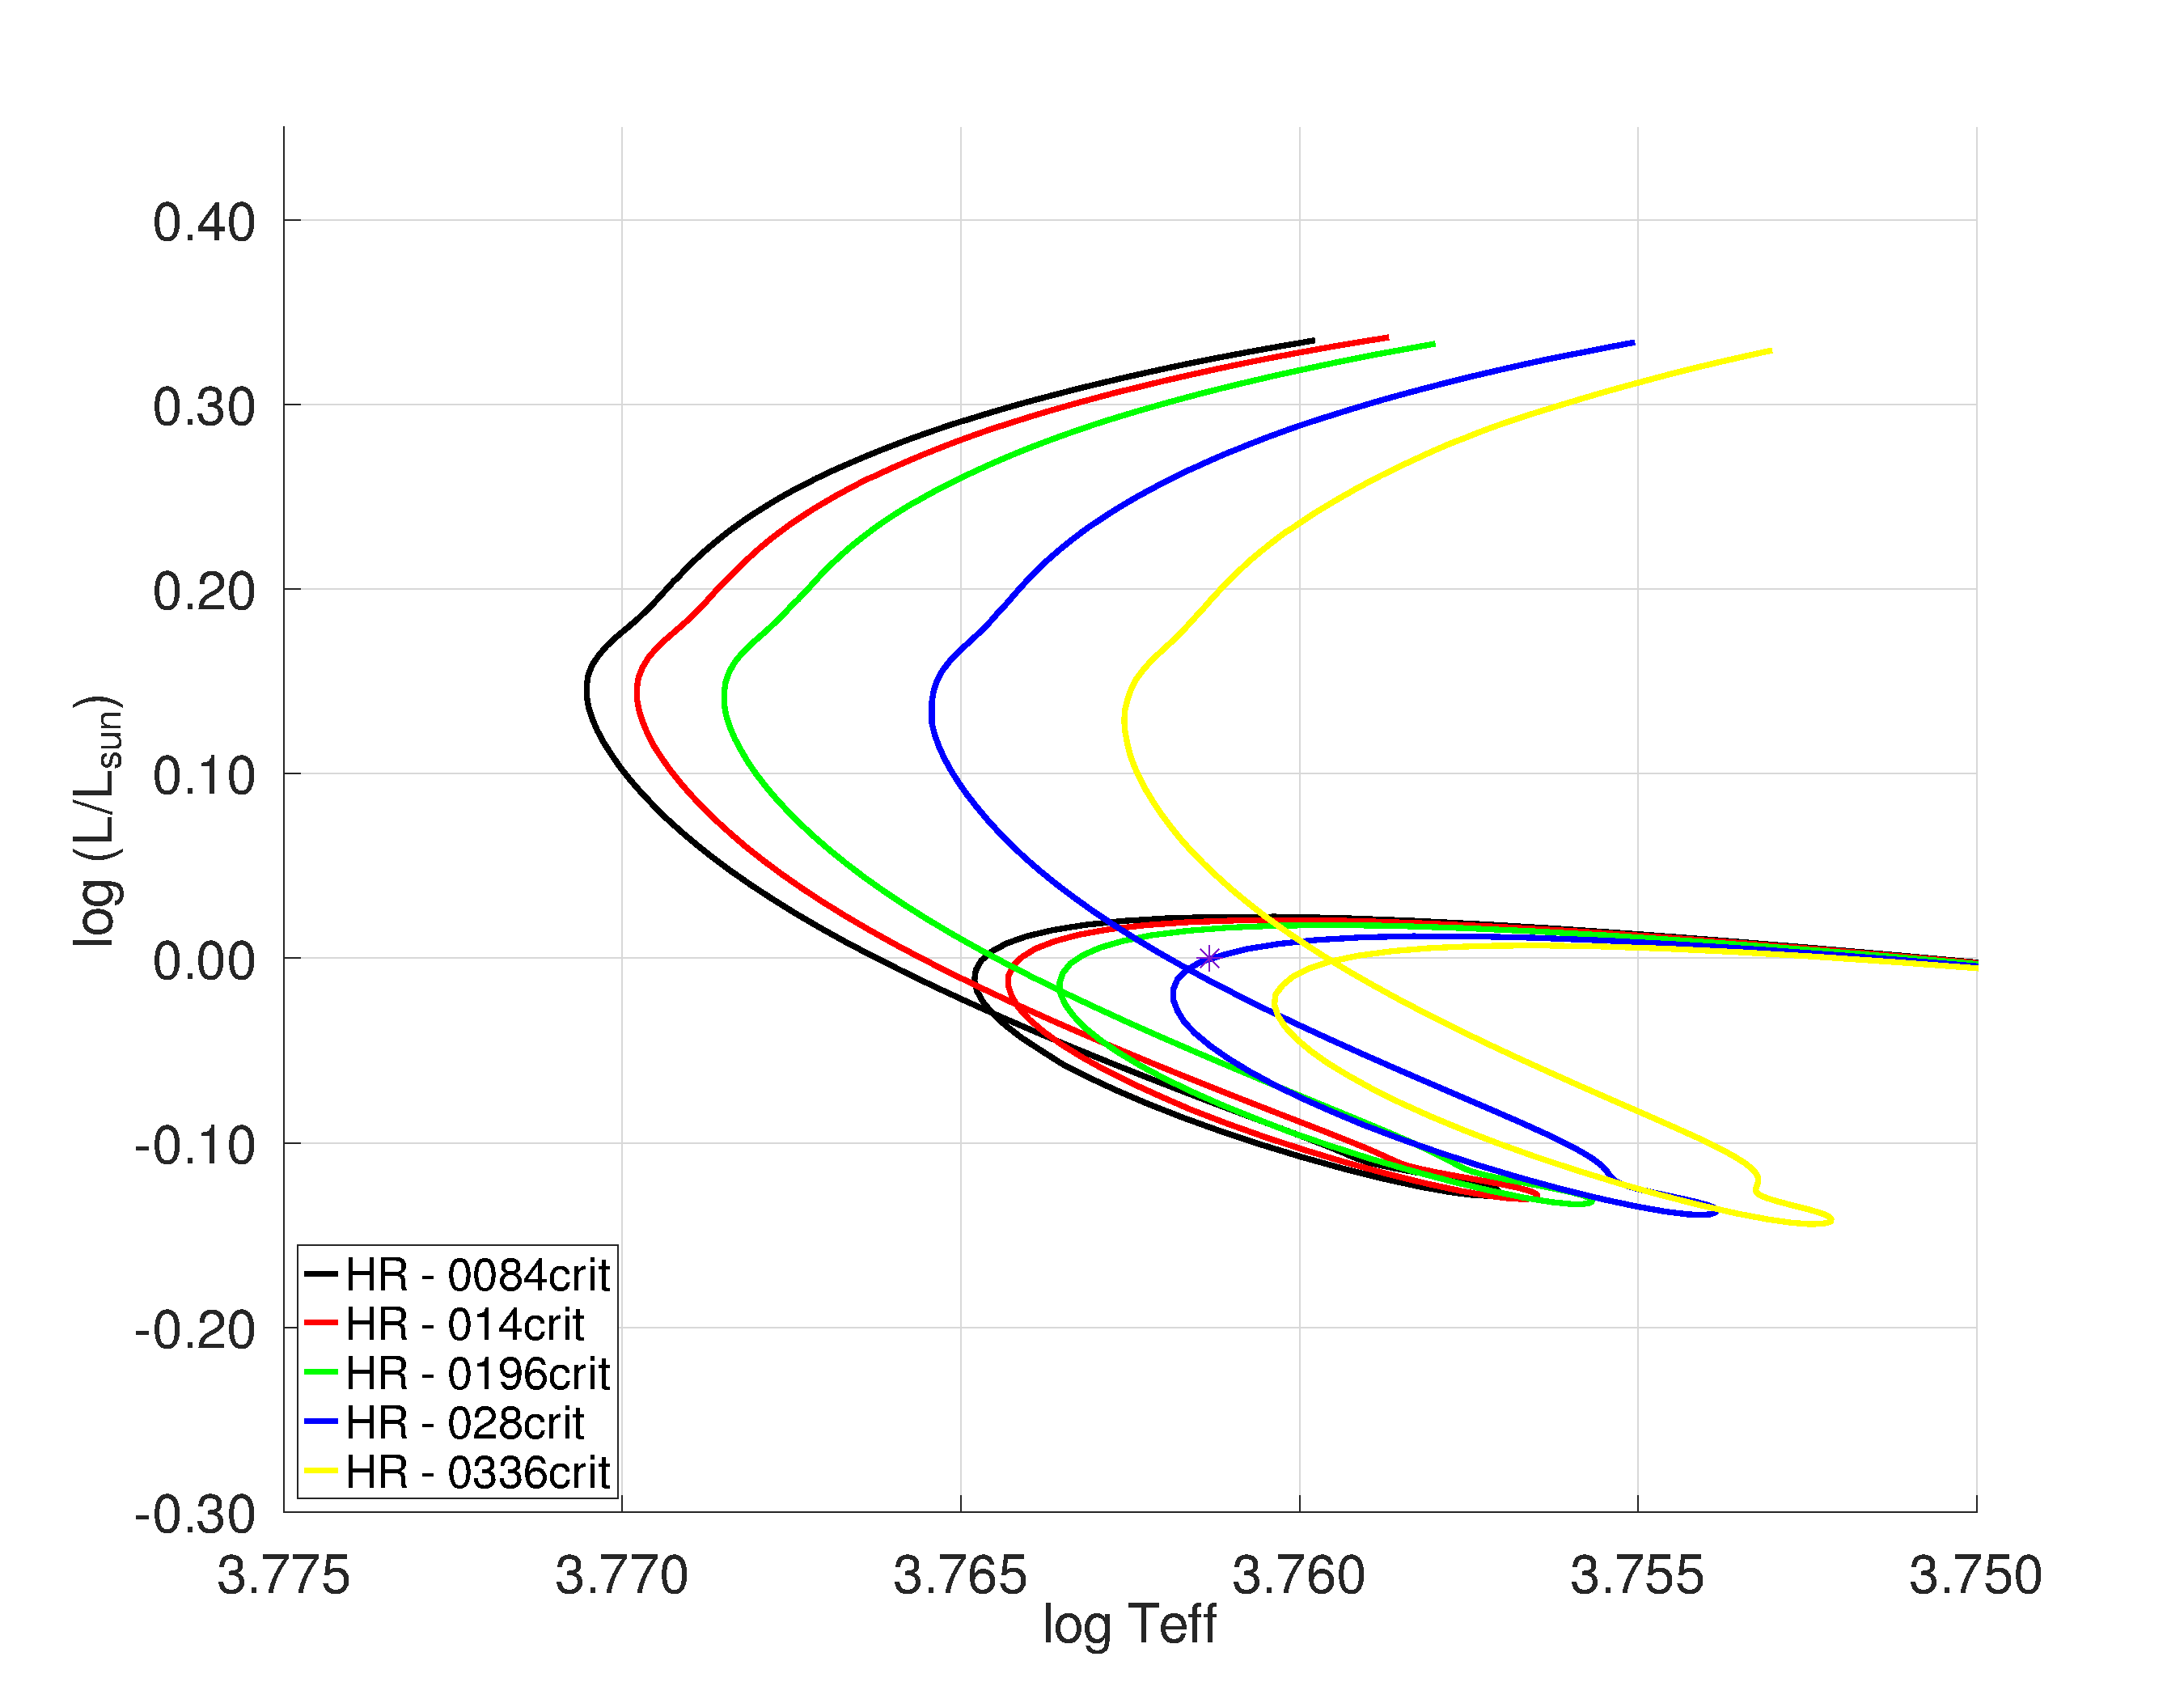
\includegraphics[width=0.7\textwidth]{img/paper2/hr_var_vel_0_0g_z10.pdf}
	\caption{Similar a la Figura \ref{fig:hr_var_vel_var_g_z13} pero mostrando ahora las trayectorias evolutivas estelares en ausencia (0G) de un campo magnético. La rotación se activa en los modelos en el PMS y esos modelos llegan antes a la ZAMS y a un $\teff$ menor que el que no rota (línea negra sólida). La luminosidad se expresa en términos de $\lsun$. $\lsun$ = 3.761. (Figura tomada de \cite{Caballero2020}.)}
	\label{fig:hr_var_vel_0g}
\end{figure}

La figura \ref{fig:teff_logg_var_vel_g3} muestra cómo se comportan $\teff$ y $\gsurf$ a lo largo de la evolución de los modelos. Para aquellos con una mayor velocidad de rotación, observamos que tanto su temperatura como su gravedad superficial son menores que en los modelos de rotación más lenta, en consonancia con el oscurecimiento de la gravedad. Cabe destacar que en la fase de aproximación ZAMS observamos para el modelo de rotación más rápida (amarillo) que su gravedad superficial es mayor que la del resto de modelos más lentos. Esto puede explicarse observando la Figura \ref{fig:lograd_var_vel_g3}, que muestra la evolución del radio estelar para los distintos modelos, en función del tiempo y $\omegaini$. Alrededor del intervalo de $2.5x10^{7}$ y $3.5x10^{7}$ Ga (delimitado por las líneas cian) y después de la ZAMS, desde alrededor de $5.4x10^{7}$ a $11.2x10^{7}$ Ga (delimitado por las líneas magenta) el radio estelar del modelo más rápido es menor que el del resto, produciendo un $\gsurf$ mayor, y esto a su vez significa una menor pérdida de masa (véase la Fig. \ref{fig:mdot_var_vel_g3}). Durante este período el modelo más rápido lo hace a un ritmo menor y expone una gravedad superficial mayor. Recordemos que el radio estelar tiene una influencia inversamente cuadrática en el valor de $\gsurf$. Esta "anomalía" desaparece en cuanto el radio estelar vuelve a ser mayor para el modelo más rápido.\par


\begin{figure}
	\centering
	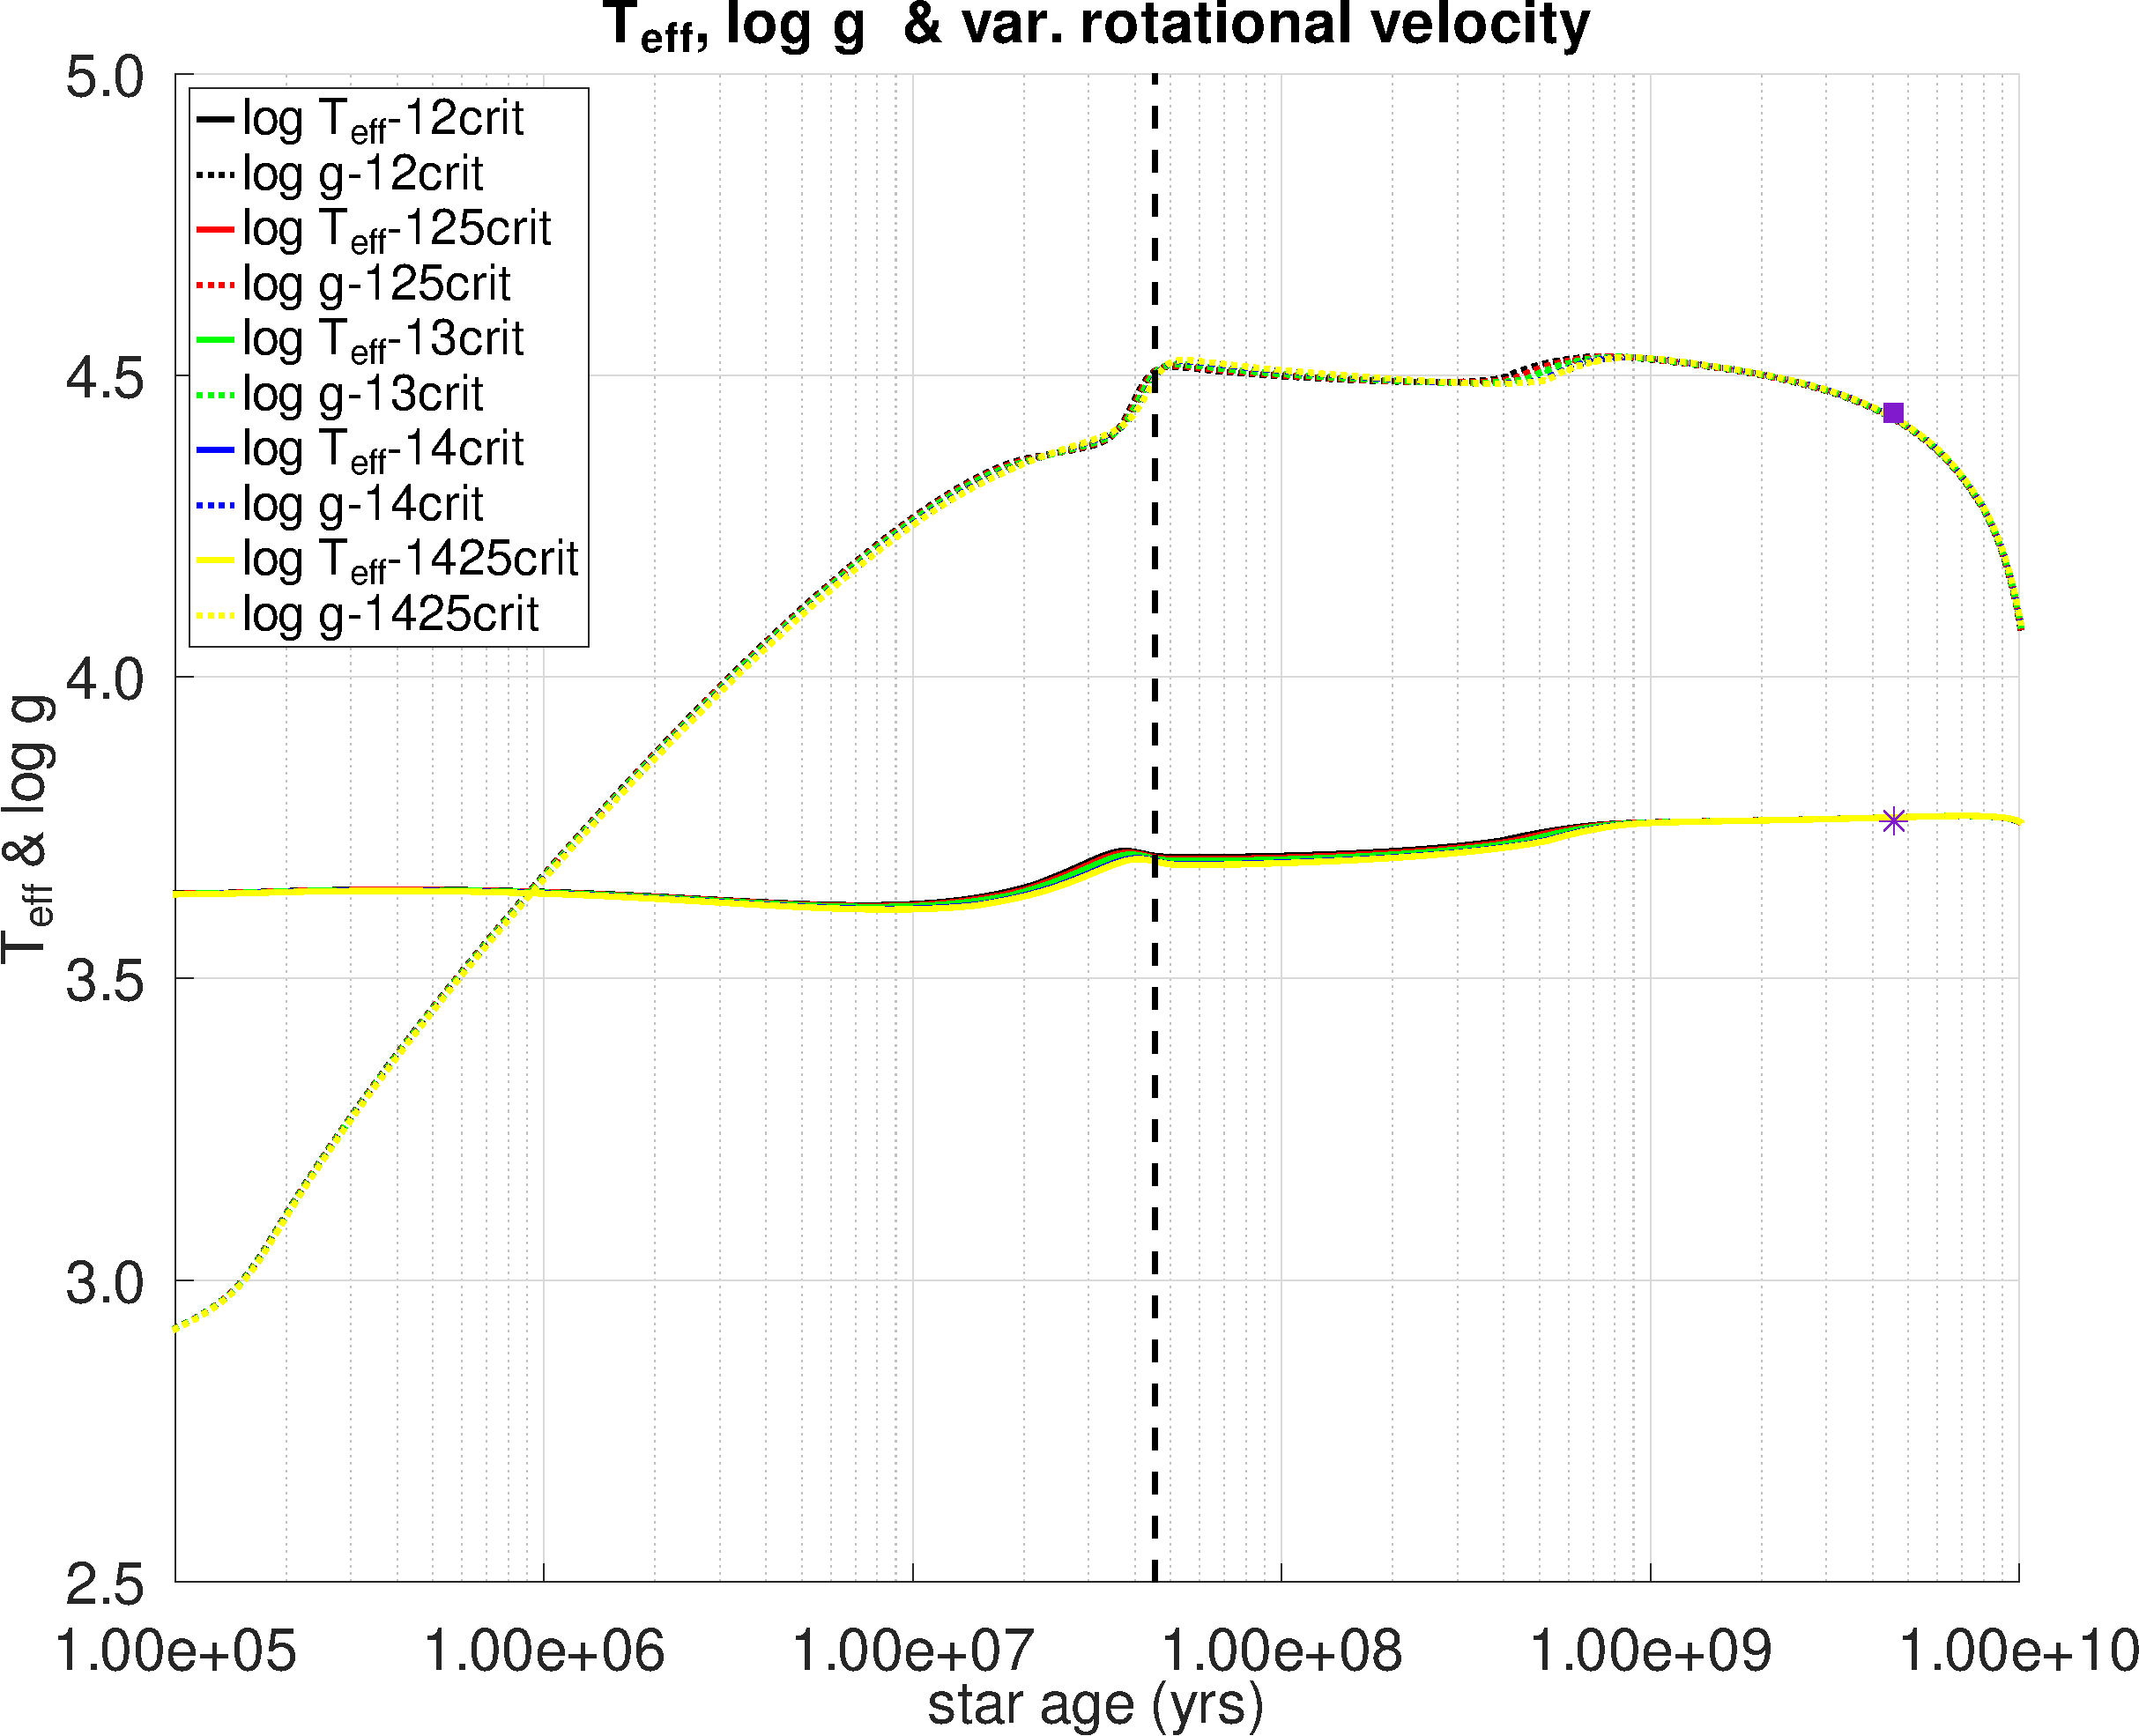
\includegraphics[width=0.7\textwidth]{img/paper2/teff_logg_var_vel_g3.pdf}
	\caption{La evolución de $\teff$ y $\gsurf$, en función del tiempo y $\omegaini$ para varios modelos de 1 $\msun$. Los modelos incluyen una rotación inicial con $\omegaini$ entre 0.12 y 0.1425. Los intervalos de edad [$2.5x10^{7},3.5x10^{7}$] Ga y [$5.4x10^{7},11.2x10^{7}$] Ga, delimitados por las líneas cian y magenta respectivamente, destacan periodos en los que el modelo más rápido con $\omegaini$=0,1425 expone una gravedad superficial superior a la del resto de los más lentos. La estrella morada es el $\teff$, y el cuadrado morado es la $\gsurf$ para el Sol actual \cite{Gill2012}. La línea vertical discontinua hace referencia a la ZAMS.}
	\label{fig:teff_logg_var_vel_g3}
\end{figure}

\begin{figure}
	\centering
	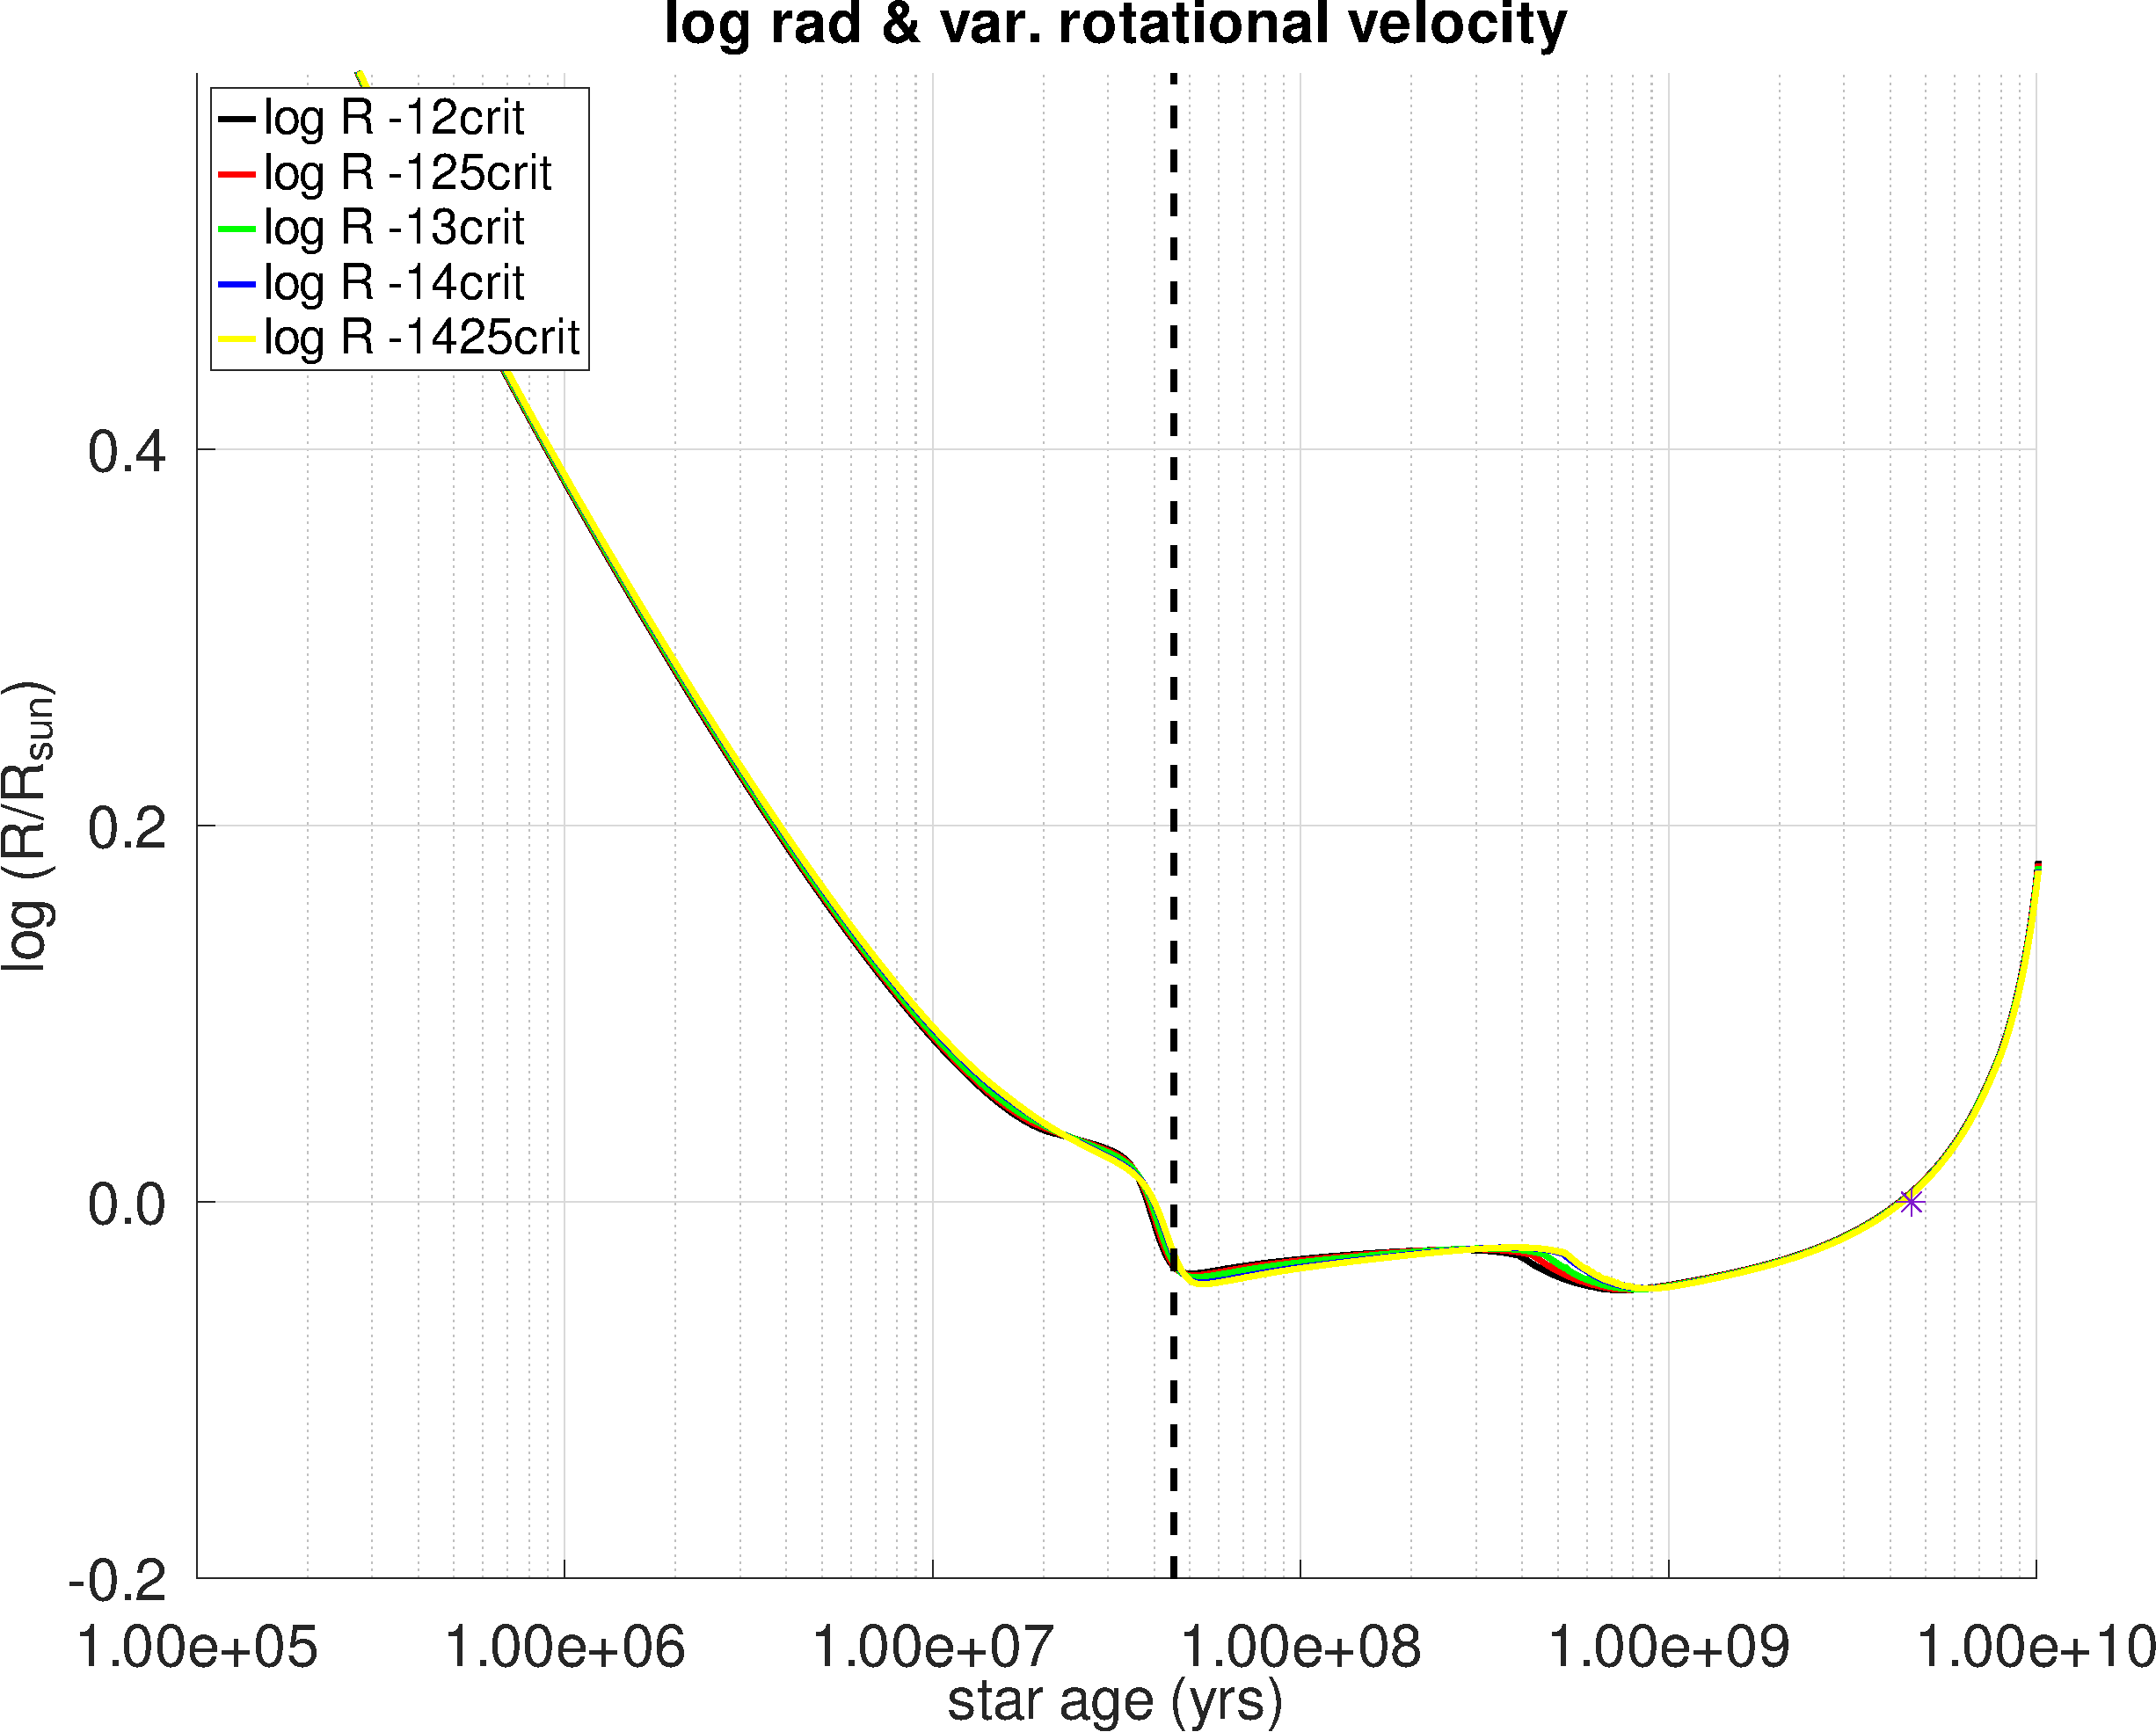
\includegraphics[width=0.7\textwidth]{img/paper2/lograd_var_vel_g3.pdf}
	\caption{La evolución del radio estelar, en función del tiempo y $\omegaini$ para varios modelos de 1 $\msun$ y sus. Los modelos incluyen rotación inicial con $\omegaini$ entre 0.12 y 0.1425. La estrella púrpura es el radio para el Sol actual \cite{Gill2012}. La línea vertical discontinua hace referencia a la ZAMS.}
	\label{fig:lograd_var_vel_g3}
\end{figure}


\section{Comparativa MB intensidad fija vs variable}
\section{Conclusiones}

\endinput
%--------------------------------------------------------------------
% FIN DEL CAPÍTULO. 
%--------------------------------------------------------------------

